
%% bare_jrnl.tex
%% V1.4b
%% 2015/08/26
%% by Michael Shell
%% see http://www.michaelshell.org/
%% for current contact information.
%%
%% This is a skeleton file demonstrating the use of IEEEtran.cls
%% (requires IEEEtran.cls version 1.8b or later) with an IEEE
%% journal paper.
%%
%% Support sites:
%% http://www.michaelshell.org/tex/ieeetran/
%% http://www.ctan.org/pkg/ieeetran
%% and
%% http://www.ieee.org/

\documentclass[journal]{IEEEtran}

% *** PACKAGES ***
\usepackage{algorithm, algorithmic}
\usepackage{amsmath}
\usepackage{amssymb}
\usepackage{amsthm}
\newtheorem{assumption}{Assumption}
\usepackage{booktabs}
\usepackage[noadjust]{cite}
\usepackage{caption}
\usepackage{color}
\usepackage{enumerate}
\usepackage{mathtools}
\usepackage{multirow}
\usepackage{url}

% *** GRAPHICS RELATED PACKAGES ***
%
\ifCLASSINFOpdf
\usepackage[pdftex]{graphicx}
  % declare the path(s) where your graphic files are
 \graphicspath{{../Figures}}
  % and their extensions so you won't have to specify these with
  % every instance of \includegraphics
  \DeclareGraphicsExtensions{.pdf,.jpeg,.png}
  \else
  % or other class option (dvipsone, dvipdf, if not using dvips). graphicx
  % will default to the driver specified in the system graphics.cfg if no
  % driver is specified.
  % \usepackage[dvips]{graphicx}
  % declare the path(s) where your graphic files are
  % \graphicspath{{../eps/}}
  % and their extensions so you won't have to specify these with
  % every instance of \includegraphics
  % \DeclareGraphicsExtensions{.eps}
\fi

% correct bad hyphenation here
%\hyphenation{op-tical net-works semi-conduc-tor}

\begin{document}
% Do not put math or special symbols in the title.
\title{Multi-Target Tracking\\ via Mixed Integer Optimization}


% author names and IEEE memberships
\author{Dimitris~Bertsimas,~Zachary~Saunders, and Shimrit~Shtern}

% make the title area
\maketitle

% As a general rule, do not put math, special symbols or citations
% in the abstract or keywords.
\begin{abstract}
The field of multi-target tracking faces two primary challenges: (i) data association and (ii) trajectory estimation. MTT problems are well researched with many algorithms solving these two problems separately, however few algorithms attempt to solve these simultaneously and even fewer utilize optimization. In this paper we introduce a new mixed integer optimization (MIO) model which solves the data association and trajectory estimation problems simultaneously by minimizing an easily interpretable global objective function. Furthermore, we propose a greedy heuristic which quickly finds good solutions. We extend both the heuristic and the MIO model to scenarios with missed detections and false alarms. 
\end{abstract}

% Note that keywords are not normally used for peer review papers.
\begin{IEEEkeywords}
optimization; multi-target tracking; data association; trajectory estimation; mixed integer optimization 
\end{IEEEkeywords}

\section{Introduction}\label{sec: Intro}
\IEEEPARstart{M}{ulti}-target tracking is the problem of estimation the state of multiple dynamic objects, referred to as \textit{targets} over a fixed window of time. At various points of time within the window, the targets are observed in a \textit{scan}, resulting in set of \textit{detections}. From these detections, the multi-target tracking problem aims to extract information about target dynamics. 

Solutions to this problem are sought across many civilian and military applications including but not limited to ballistic missile and aircraft defense, space applications, the movement of ships and ground troops, autonomous vehicles and robotics, and air traffic control. Each application has unique attributes and assumptions, and various algorithms have been developed for each. As a result, the field of multi-target tracking has expanded to numerous research venues, and there is a wide range of literature on the topic. A more complete overview of all MTT methods, including the classes of algorithms and their variants as well as additional methods not discussed in this paper, can be found in \cite{MTT-Taxonomy}. For a more exhaustive overview of estimation techniques, filtering, gating, and more please see \cite{Bar-Shalom_MTT} or \cite{Bar-Shalom_Estimation}.

The field of multi-target tracking faces two primary challenges: (i) data association and (ii) trajectory estimation.  Given a set of sensor detections the data association problem consists of assigning the detections to a set of targets. Alternatively, this can be viewed as a labeling problem in which each detection needs to be labeled with a target identifier. The association problem is further complicated when sensors fail to report detections (missed detection) or incorrectly report detections (false alarm), resulting in ambiguity in the number of existing targets. The trajectory estimation problem consists of estimating the state space of a target (\textit{i.e.}, position, velocity, acceleration, size, etc.) from the associated detections of the aforementioned assignment problem. Even when all of the associations are known, the estimation problem is challenging due to the presence of measurement noise. As can be seen, the two problems of data association and trajectory estimation are closely related and dependent on one another. 

Some classical algorithms treat the data association and trajectory estimation problems separately using a combination of probabilistic approaches to determine data associations and filters to estimate trajectories. One such algorithm is the global nearest neighbor (GNN). The GNN algorithm is a naive 2-D assignment algorithm, which evaluates one scan of detections at a time, globally assigning the nearest detection at each scan \cite{GNN}. Once the data association has been determined, the detections are often passed through one of numerous filters, most commonly a Kalman filter \cite{Kalman}, which updates the trajectory estimates before the algorithm progresses forward to the next scan. This process repeats sequentially through each scan of data.

Modern algorithms in the field of multi-target tracking are most commonly statistical based, often relying on heavy probabilistic assumptions about the underlying target dynamics or detection process. The two most prevalent statistical algorithms in the field of multi-target tracking are the the Multiple Hypothesis Tracker (MHT) and the Joint Probability Data Association Filter (JPDAF) and their numerous variants and extensions. Both classes of algorithms attempt to solve the data association problem by generating a set of potential hypotheses, or possible detection-to-track assignments. Here a \textit{track} is a set of labelled detections belonging to the same target. Probabilities are assigned to each hypothesis based on the likelihood of the trajectory's existence, and numerous approaches for accomplishing this task have been proposed.

The MHT, first proposed by Reid in \cite{MHT-Seminal}, assigns likelihood values to hypotheses using a Bayesian MAP estimator, which requires assumptions on object dynamics. This algorithm is generally considered to be the modern standard for solving the data association problem. Many variants have been proposed for implementation which leverage techniques such as clustering, gating, hypothesis selection, hypothesis pruning, and merging of state estimates. Many of these methods are summarized by Blackman in \cite{MHT-Overview}. 

While the MHT has seen various forms of success, it faces several key challenges. Namely, the curse of dimensionality and complexity. The number of possible hypotheses grows exponentially with the number of potential tracks and the number of scans. Consequently, it is considered intractable for large scenarios. Moreover, the MHT might require extensive tuning and thus may be difficult to implement in practice, in addition to being computationally expensive. For these reasons it is generally considered to be one of the most complex MTT algorithms. 

A Probability Data Association (PDA) takes a Bayesian approach to solving the data association problem by finding detection-to-target assignment probabilities via a posterior PDF, which again requires heavy assumptions on object dynamics and the detection process. In similar fashion, a Joint PDA (JPDA) assigns probabilities that are computed \textit{jointly} across all targets. The JPDAF is an algorithm which implements the JPDA along with filters and estimation methods as discussed previously. \cite{Bar-Shalom_MTT} 

A limited number of optimization based algorithms have been applied to solve the MTT problem, most of which attempt to solve by mapping the measurement set onto a trellis and seek the optimal measurement association sequence. Some examples include the Multi-Target Viterbi\cite{Viterbi-1} and an extension in \cite{Viterbi-2} which formulates \cite{Viterbi-1} as a network flow, reducing the solve time from exponential to polynomial. Others have suggested adaptations which allow this approach to be used similar to MHT methods by outputting a single best set of K tracks, or a list of L best sets of k tracks \cite{Viterbi-3}. 

Compared to the number of statistical based algorithms in the MTT literature, optimization based algorithms are relatively lacking. In fact, most occurrences of optimization in the MTT literature propose the use of optimization to leverage statistical algorithms, in particular the MHT. For example, Integer optimization has been used to improve MHT hypothesis selection by solving an assignment problem which chooses the best hypothesis, but only after costs have been assigned (statistically based) and hypotheses have been pruned \cite{MHT-IP}. Somewhat similarly, linear optimization has also been used to assist in the hypothesis selection process for the MHT \cite{MHT-LP}. Still, other attempts aim to improve the MHT hypothesis selection process via Lagrangian relaxation \cite{Lagrangian}. 

More recently, Andriyenko and Schindler have proposed formulating the MTT problem as a minimization of a continuous energy in \cite{Continuous_energy} and then again as a minimization of discrete-continuous energy in \cite{Discrete-Continuous_energy}. These algorithms aim to more accurately represent the nature of the problem, but sacrifice interpretability for complexity in the process. Rather than formulating the problem to lend it easily to traditional global optimization methods, the authors intend to leverage the use of optimization techniques to find strong local minima of their proposed energy objective, and they achieve strong results in doing so. However, this approach calls for the use of several parameters that must be tuned and few recommendations are provided for how to go about such a tuning process. Additionally, these methods require initialization heuristics to begin the solving process, which is in itself complicated to implement and is not directly connected to the optimization problem solved. 

In this paper we propose the use of mixed integer optimization (MIO) to formulate and solve the multi-target tracking problem. Although MIOs are generally thought to be intractable (NP-Hard), in many practical cases near optimal solutions and even optimal solutions to these problems can be obtained in reasonable time \cite{Computation}. This can be attributed to the fact that MIO solvers have seen significant performance improvements in recent years due to advancements in both methodology and hardware. The development of new heuristic methods, discoveries in cutting plane theory, and improved linear optimization methods have all contributed to improvements in performance \cite{Gurobi-MIP}. Modern solvers such as Gurobi and CPLEX have been shown to perform extremely well on benchmark tests. In the past six years alone, Gurobi has seen performance improvements by a factor of 48.7 \cite{Gurobi-Benchmark}. CPLEX saw improvements by a factor of 29,000 from 1991 to 2007 \cite{CPLEX-Benchmark}. From 1994 to 2014, the growth of supercomputing power as recorded by the TOP500 list has improved by a factor of 567839 \cite{Supercomputer}. Thus, the total combined effective improvement of software and hardware advancements is on the scale of 800 billion times in the past 25 years. 

The literature is also lacking in performance metrics for the evaluation of MTT algorithms. There is no standard method of measuring scenario complexity or algorithm performance as a function of this complexity. In many cases only the sensor's detection noise is taken into account and other factors such as target density is negated. Recent work \cite{MTT-Performance} proposes a mathematically rigorous performance metric for measuring the distance between ground truth and estimated track, but there is not much attention given to the complexity of generated scenarios. In this paper we also suggest measures of complexity and performance which are related to the ones suggested in \cite{MTT-Performance} but we show the value in relating a complexity measure to performance measures, namely that it allows you to evaluate the data association and trajectory estimation problems separately. We evaluate the methods suggested in this paper using these complexity and performance measures on two simulated experiments.

The main contributions of this paper are as follows: 
\begin{enumerate}[(i)]
\item We introduce a simple interpretable MIO model which solves the data association and trajectory estimation problems simultaneously for a sensor with no detection ambiguity. The model does not require to tuning of parameters. This MIO is tractable, in the sense that it can be solved to optimality or near optimality in a reasonable amount of time, for the considered applications.
\item We propose a heuristic, motivated by the optimization problem, which gives us feasible solutions to this problem and show how it can be used as warm start to the MIO in order to improve the quality of the solutions obtained as well as the running time. 
\item We extend this basic MIO model and corresponding heuristic initialization algorithm for the case of detection ambiguity, i.e., the case where there are both missed detections and false alarms, keeping interpretability while only adding two tunable parameters, as well as provide general guidelines as how to tune these parameters. 
\item  We present a new measure of complexity for the data association problem, and show how allows scenario generation and performance to be measured separately in each of their own natural demands. We also discuss a simplified measure of performance for the trajectory estimation problem. 
\end{enumerate}

The paper structure is as follows. We begin with a description of the MTT problem as we wish to model it in Section~\ref{sec:Problem Description}. In Section~\ref{sec:Basic MIO Model} we develop a simple MIO formulation for a sensor with no detection ambiguity and extend it to a generalized formulation. Following is a discussion on a proposed heuristic in Section~\ref{sec:Heuristic}. Then we propose extensions for both the MIO formulation and the heuristic to a sensor with detection ambiguity in Section~\ref{sec:Robust MIO Model}. Metrics for measuring scenario complexity and algorithm performance are proposed in Section~\ref{sec:Scenario-Performance}.  Experimental methodology and a summary of significant computational results are discussed in Section~\ref{sec:Basic_Results}. An extension of the experiment and results are made to the scenarios with detection ambiguity in Section~\ref{sec:Robust_Results}. Finally, conclusions and future work are discussed in Section~\ref{sec:Conclusion}.

{\bf General Notations:}
Unless specified otherwise, $\|\cdot\|$ is used to indicate the L1 norm, and $|\cdot|$ refers to element wise absolute value.

\section{Problem Description}\label{sec:Problem Description}
In this paper, we restrict our exploration of the MTT problem to the automatic tracking of multiple, independent point targets using a single sensor. A \textit{target} is the object of interest. A point target's only identifiable attributes are its state space, which we restrict to position and velocity. The state space fully defines the field of \textit{trajectories}, or paths along which targets travel. A \textit{detection} is collected from each target at sequential scans. Detections are subject to noise. We treat two general scenarios: with and without detection ambiguity. 

When there is no detection ambiguity, the sensor produces exactly one detection for each target in each scan, and there is no other source of detections. Therefore, the number of detections in each scan exactly equals the number of targets in existence. Under these conditions the data association problem reduces to a one-to-one assignment problem. Our basic optimization model, presented in Section~\ref{sec:Basic MIO Model} aims to model this variant of the MTT problem.

Detection ambiguity refers to the more complex case where the sensor generates both false alarms and missed detections. A \textit{false alarm} occurs when a detection is collected when in fact no target exists. This could be the result of measurement error or difficulties in signal processing. A \textit{missed detection} occurs when a data point is not collected in a given scan where a target does in fact actually exist. Now, the number of detections in each scan could be higher or lower than the actual number of existing targets. Under these conditions, each detection can now be assigned to a target in the same manner as before, or the detection can be classified as a false alarm. Furthermore, we wish to identify the location (scan and target ID) of a missed detection. In Section~\ref{sec:Robust MIO Model} we make extensions of the formulation of our basic optimization model to a robust formulation that deals with this detection ambiguity, and we will refer to this formulation as the robust MIO model.

Throughout the paper we make the following assumptions:
\begin{assumption}\label{ass:general_assumption}
\begin{enumerate}[(i)]
\item{}All targets have constant velocity. \textit{i.e.}, Targets do not maneuver and no outside forces act on them.
\item Each target's dynamics are independent of one another.
\item The number of targets remains constant throughout the window of observation, \textit{i.e.}, there is no birth/death of targets.
\item Each target produces at most one detection per scan.
\item The detection errors are independent of one another.
\end{enumerate}
\end{assumption}

{\bf Notation:}
We observe $P$ targets over a fixed time window in which $T$ scans are collected. Scans occur at a fixed rate of 1Hz, such that the set of scans can be time stamped by $\{t_{1}, t_{2},...,T\}. $ The $i^{th}$ detection of the $t^{th}$ scan is indicated by $x_{it}$, such that a scan of data at time \textit{t} is the unordered set of detections $\mathcal{X}_{t} = \{x_{1t}, x_{2,t},...,x_{P,t}\}$. The data for the problem is the ordered set of scans $\boldsymbol{\mathcal{X}}=\{\mathcal{X}_{1},\mathcal{X}_{2},...,\mathcal{X}_{T}\}$. The state space of target trajectories is paramatarized by a true initial position $\alpha^{\text{true}}_{j}$ and a true constant velocity $\beta^{\text{true}}_{j}$. Therefore, the true position $\bar{x}_{jt}$ of trajectory $j$ at scan $t$ is given by: 

\begin{align}
	\bar{x}_{jt} = \alpha^{\text{true}}_{j} + \beta^{\text{true}}_{j}t
\end{align}

\section{Basic MIO Model}\label{sec:Basic MIO Model}
In this section, we deal with the case of no detection ambiguity. Therefore, we add the following, more restrictive assumptions, to those presented in Assumption~\ref{ass:general_assumption}
\begin{assumption}\label{ass:basic_assumptions}
\begin{enumerate}[(i)]
\item The sensor generates exactly one detection for each target at each time (no missed detections).
\item The sensor does not generate any additional detections (no false alarms).
\end{enumerate}
\end{assumption}

We begin constructing our MIO model by defining decision variables that represent the desired detection to target associations and target estimated trajectories. Next, using these decision variables, we develop an objective function which mathematically quantifies the value of the model decisions, in this case as a measure of distance of the estimated trajectories from the associated detections. Finally, we restrict these variables using constraints that force the model to find solutions that are feasible for the MTT problem. The model is developed step by step in the coming sections before the full model is presented. 

\subsection{Decision Variables}
The data association and trajectory estimation problems require unique decision variables. Because these two problems lie in different domains, the variables we use to represent these decisions also differ. First, we introduce \textit{continuous} decision variables $\alpha_{j} \in \mathbb{R}^n$ and $\beta_{j} \in \mathbb{R}^n$ to represent the estimated initial position and velocity of each trajectory \textit{j}.  In our interpretation of the MTT problem we allow the trajectory parameters to lie anywhere in the real-continuous domain. For the data estimation problem, we wish to assign detections to trajectories, a naturally discrete problem. Therefore, we introduce binary decision variables $y_{itj}$ to indicate whether detection $x_{it}$ is assigned to trajectory \textit{j} or not:

\begin{align}
y_{itj} =
\begin{cases}
1, & \text{if detection $x_{it}$ is assigned to trajectory \textit{j},} \\
0, & \text{otherwise.}
\end{cases}
\end{align}

\subsection{Objective Function}
Next, we would like to develop a function which accurately scores the quality of a feasible solution. An ideal objective function would jointly provide a single quantifiable measure of goodness for both the data association and trajectory estimation problems. Therefore we want the objective to take into account the assignments of detections in addition to the estimated trajectory determined by those assignments.

In terms of our established decision variables, the estimated position of the linear trajectory \textit{j} at time \textit{t} is given by:

\begin{align}\label{eq:estimate_pos}
	\hat{x}_{jt} =  \alpha_{j} + \beta_{j}t
\end{align}

For the trajectory estimation problem we wish to minimize the distance between $x_{it}$ and $\hat{x}_{jt}$. In other words, for detections $x_{it}$ assigned to trajectory $j$, we wish to minimize $\|x_{it} - \hat{x}_{jt}\|$ for some norm. The two natural norms to consider here are the L1 and L2 norms. The L1 norm has the advantage that it can be reformulated using linear optimization (through the addition of continuous variables and constraints), and it is well known to be more robust to outliers. Furthermore, existing algorithms for MIO are more well developed for linear rather than quadratic optimization. However, the L2 norm square form (RSS) has the advantage that it can be quickly computed using a matrix formulation, making it more predisposed to a heuristic. This concept will be discussed further in section~\ref{sec:Heuristic}.

Substituting \eqref{eq:estimate_pos} for $\hat{x}_{jt}$ we arrive at our objective function:
\begin{align}
\underset{\alpha_{j}, \beta_{j}}{\text{minimize: }} & \sum_{(i,j)\in \mathcal{A}} \sum_{t=1}^{T} \|x_{it} - \alpha_{j} - \beta_{j}t\| 
\end{align}
where $\mathcal{A}$ is the set of pairs that indicate the assignment of detection \textit{i} to trajectory \textit{j}.
 
For the data association problem, we wish to only penalize the objective function when detection $x_{it}$ has been assigned to trajectory \textit{j}, which occurs when $y_{itj}=1$. An easy method to enforce this using our established variables would be to construct an interaction term like in \eqref{eq:simple_objective} below. 

\begin{align}\label{eq:simple_objective}
\underset{y_{itj}, \alpha_{j}, \beta_{j}}{\text{minimize: }} & \sum_{i=1}^{P} \sum_{t=1}^{T} |y_{itj}x_{it} - \alpha_{j} - \beta_{j}t\|
\end{align}

We now show that this objective can formulated using linear optimation in the case of the L1 norm by introducing continuous variables $\psi_{jt}$ and the following additional constraints. 

\begin{align}
y_{itj}x_{it} - \alpha_{j} - \beta_{j}t \leq \psi_{jt} \qquad \forall i,j,t\\
-(y_{itj}x_{it} - \alpha_{j} - \beta_{j}t) \geq \psi_{jt} \qquad \forall i,j,t
\end{align}

The resulting objective function for the case of the L1 norm would then be:
\begin{align}
\underset{\psi_{jt}}{\text{minimize: }} & \sum_{j=1}^{P} \sum_{t=1}^{T} \psi_{jt}
\end{align}
where $e$ is the vector of ones. 

For the case of the L2 norm, the objective function would be:
\begin{align}
\underset{\psi_{jt}}{\text{minimize: }} & \sum_{j=1}^{P} \sum_{t=1}^{T} {\|\psi_{jt}\|}^{2}_{2}
\end{align}

\subsection{Constraints}
For each scan, each detection $x_{it}$ must be assigned to exactly one target \textit{j}:
\begin{align}
\sum_{j=1}^{P} y_{itj} = 1 \qquad \forall i,t
\end{align}

Similarly, for each scan, each target must be assigned exactly one detection:
\begin{align}
\sum_{i=1}^{P} y_{itj} = 1 \qquad \forall j,t
\end{align}

\subsection{Simple Formulation}
Combining all of these elements together, we arrive at the following MIO model:
\begin{align*}
\underset{\psi_{jt}}{\text{minimize: }} & \sum_{j=1}^{P} \sum_{t=1}^{T} \psi_{jt} \\
\text{subject to: }	& \sum_{j=1}^{P} y_{itj} = 1 \qquad \forall i,t\\
				& \sum_{i=1}^{P} y_{itj} = 1 \qquad \forall j,t\\
				& y_{itj}x_{it} - \alpha_{j} - \beta_{j}t \leq \psi_{jt} \qquad \forall i,j,t\\
				& -(y_{itj}x_{it} - \alpha_{j} - \beta_{j}t) \geq \psi_{jt} \qquad \forall i,j,t\\
			 	& y_{itj} \in \{0,1\} \quad \forall i,t,j\\
				& \alpha_{j} \in \mathbb{R}^n \quad \forall j,\quad \beta_{j} \in \mathbb{R}^n \quad \forall j, \quad z_{jt} \in \mathbb{R}^n \quad \forall j,t
\end{align*}

\subsection{Generalized Formulation}
The previous formulation, although simple and easily interpretable, has the disadvantages of being (\textit{i}) dense and (\textit{iI}) ill suited for extension to detection ambiguity. Therefore, next, we present a generalized formulation which can be linearized through the introduction of additional binary decision variables. Alternatively, we can create a new variable $z_{jt}$ which takes on the value $x_{it}$ when $y_{ijt}=1$ and some arbitrary number when $y_{itj}=0$. Using this method we must adjust the objective function below. 

\begin{align}\label{eq:generalized_objective}
\underset{z_{jt}, \alpha_{j}, \beta_{j}}{\text{minimize: }} & \sum_{j=1}^{P} \sum_{t=1}^{T} \|z_{jt} - \alpha_{j} - \beta_{j}t\|
\end{align}

This objective can then be linearized by again introducing $\theta{jt}$ and similar constraints as follows. 
\begin{align}\label{eq:generalized_linear_objective}
\underset{\psi_{jt}}{\text{minimize: }} & \sum_{j=1}^{P} \sum_{t=1}^{T} \psi_{jt}
\end{align}
\begin{align}
z_{jt} - \alpha_{j} - \beta_{j}t \leq \psi_{jt} \qquad \forall i,j,t\\
-(z_{jt} - \alpha_{j} - \beta_{j}t) \geq \psi_{jt} \qquad \forall i,j,t
\end{align}
 
Furthermore, we must ensure that the decision variable $z_{jt}$ will only take on the value of $x_{it}$ in the objective function if $x_{it}$ is assigned to target \textit{j} ($y_{itj} = 1$). We enforce this effect using the following constraint:

\begin{align}
M_{t}(1-y_{itj}) \geq |z_{jt} - x_{it}y_{itj}| \qquad \forall i,t,j\\
\end{align}

where $M_{t} = \underset{j}{\text{max}}|x_{it}|$ for each scan. Furthermore, we can write this equivalently as a linear optimization problem by using the following set of two linear constraints:

\begin{align}
x_{it}y_{itj} + M_{t}(1-y_{itj}) \geq z_{jt} \qquad \forall i,t,j\\
x_{it}y_{itj} - M_{t}(1-y_{itj}) \leq z_{jt} \qquad \forall i,t,j
\end{align}

Combining all of these elements together, we arrive at the following generalized MIO model:
\begin{align*}
\underset{\psi_{jt}}{\text{minimize: }} & \sum_{j=1}^{P} \sum_{t=1}^{T} \psi_{jt} \\
\text{subject to: }	& \sum_{j=1}^{P} y_{itj} = 1 \qquad \forall i,t\\
				& \sum_{i=1}^{P} y_{itj} = 1 \qquad \forall j,t\\
				& x_{it}y_{itj} + M_{t}(1-y_{itj}) \geq z_{jt} \qquad \forall i,t,j\\
				& x_{it}y_{itj} - M_{t}(1-y_{itj}) \leq z_{jt} \qquad \forall i,t,j\\
				& z_{jt} - \alpha_{j} - \beta_{j}t \leq \psi_{jt} \qquad \forall i,j,t\\
				& -(z_{jt} - \alpha_{j} - \beta_{j}t) \geq \psi_{jt} \qquad \forall i,j,t\\
			 	& y_{itj} \in \{0,1\} \quad \forall i,t,j\\
				& \alpha_{j} \in \mathbb{R}^n \quad \forall j,\quad \beta_{j} \in \mathbb{R}^n \quad \forall j, \quad z_{jt} \in \mathbb{R}^n \quad \forall j,t
\end{align*}

\section{Heuristic} \label{sec:Heuristic}
Next, we present a detailed description of a heuristic which finds good feasible solutions. These solutions can be used as a warm start to the MIO, providing a performance boost to the MIO. The heuristic leverages the power of randomization local search methods to find locally optimal solutions. Although the heuristic takes a local search approach, we hypothesize that it will discover near optimal solutions, provide that it is initialized with enough random starting points.

An important distinction to discuss here is the difference in objective functions. As discussed before the two natural choices are the L1 and L2 norms. For the heuristic, we desire an objective which can be calculated efficiently. Therefore, in this case the L2 norm square (RSS) is the preferred choice because it can be calculated quickly using matrix algebra. \cite{RSS-Matrix} shows how RSS can be quickly computed using linear algebra.

The algorithm initializes by randomizing a solution which satisfies equations 6 and 7. The initial  parameters $\alpha_{j}$ and $\beta_{j}$ are calculated as well as the objective score, $RSS^{0}$. In swap $k$ for scan $t$ choose $i,l\in \{1,\ldots,P\}$ detections and $j,m\in\{1,\ldots,P\}$ targets such that $y^k_{itj}=1$ and $y^k_{ltm}=1$. Switch the detection association so that $y^{k+1}_{ltj}=1$ and $y^{k+1}_{itm}=1$. Compute $\alpha_{j}, \beta_{j}, \alpha_{m}$, $\beta_{m}$, and $RSS^{k}$. If the objective score improves, the swap is kept, otherwise it is rejected. The algorithm then advances to the next scan where the same process is repeated, and it terminates once it makes a single pass through all scans without accepting a single switch. As we will see in the computational results section, Algorithm~\ref{alg:Basic_Heuristic} runs very efficiently, providing high quality global solutions very quickly. Furthermore, this algorithm can be parallelized by running partitions of the $N$ starting points on separate cores, leading to even greater performance advantages. A proposed pseudocode for the heuristic is provided below in Algorithm~\ref{alg:Basic_Heuristic}. 

\begin{algorithm}
 \caption{Randomized local search with heuristic swaps}
 \label{alg:Basic_Heuristic}
 \begin{algorithmic}[1]
  \renewcommand{\algorithmicrequire}{\textbf{Input:}}
  \renewcommand{\algorithmicensure}{\textbf{Output:}}
 \REQUIRE $\boldsymbol{\mathcal{X}}$, P, T
 \ENSURE  $RSS$, $y_{itj}$
 \\ \textit{Initialization} : Assign random initial assignments for $y^{0}_{itj}$
  \STATE Calculate $\alpha_{j}, \beta_{j} \quad \forall j $
  \STATE Calculate $RSS^{0}$
  \STATE swapped $\leftarrow true$
  \STATE $k\leftarrow1$
  \WHILE{swapped}
  \STATE swapped $\leftarrow false$
  \FOR{$t$ in $\{t_{1},t_{2},...,T\}$}
  \STATE Randomly choose $j,m\in\{1,\ldots,P\}$
  \STATE Find $i,l$ such that $y^{k-1}_{itm}\leftarrow1$ and $y^{k-1}_{ltj}\leftarrow1$
  \STATE Swap such that $y^{k}_{itj}\leftarrow1$ and $y^{k}_{ltm}\leftarrow1$
  \STATE Calculate $RSS^{k}, \alpha_{j}, \beta_{j}, \alpha_{m}, \beta_{m}$
  \IF {($RSS^{k} \geq RSS^{k-1}$)}
  \STATE $y^{k} \leftarrow y^{k-1}$
  \ELSE 
  \STATE swapped $\leftarrow true$
  \ENDIF
  \ENDFOR
  \STATE $ k \leftarrow k + 1 $
  \ENDWHILE
 \RETURN $RSS^{k}, y^{k}_{itj}$ 
 \end{algorithmic} 
 \end{algorithm}

\section{Robust MIO Model}\label{sec:Robust MIO Model}
In this section we treat the case of detection ambiguity. The key difference is that now the number of targets is unknown, and this becomes a third problem which we wish to solve in addition to the data association and trajectory estimation problems which remain once the number of targets has been determined. Since in this case both missed detections and false alarms are present the number of targets is unknown and we may no longer have the same number of detections at each scan. Therefore, we must introduce additional notation for this scenario. We let $n_{t}$ represent  the number of detections at time \textit{t}. We can then identify the fewest and largest number of detections in a scan with $N_{0} = \underset{t}{\text{min }} n_{t}$ and $N_{1} = \underset{t}{\text{max }}  n_{t}$, respectively. 

Specifically, in this case we replace Assumption~\ref{ass:basic_assumptions} by the following less restrictive assumptions.
\begin{assumption}\label{ass:robust_assumptions}
\begin{enumerate}[(i)]
\item The sensor does not generate a detection for any target for any time with probability $P_{d}$ which is constant and independent between targets and scans.
\item At each point in time the sensor generates false alarms according to a Poisson distribution with rate $\lambda_{FA}$, which are located uniformally in the space.
\item The number of true targets $P$ satisfies $N_0\leq P \leq N_1$.
\end{enumerate}
\end{assumption}

We first show that this problem can be solved by dividing it into a subset of simpler problems. We present a MIO formulation that assumes a fixed number of targets. This formulation allows us to leverage the power of parallelization to solve the problem by solving each subproblem separately. The results can then be gathered and compared to find the globally optimal solution. For completeness we also present a formulation which solves the original problem without the need for multiple parallelized MIOs.

\subsection{Fixed Number of Targets (P)}
If we first assume that the number of targets is fixed, we can more easily adapt the generalized formulation presented in Section III to handle the addition of false alarms and missed detections. This simple adaptation requires the introduction of two additional variable types and minimal constraint changes. We can then run these formulations for each possible value of fixed number of targets \textit{P} across the range of $N_{0}$ to $N_{1}$ and choose the solution with the best objective overall. Furthermore, this is an advantageous strategy because each independent experiment can be run in parallel. 

\subsubsection{Decision Variables}
We first introduce new binary decision variables $F_{it}$ to indicate whether or not a detection $x_{it}$ is a false alarm. 

\[F_{it} = 
\begin{cases}
1, & \text{if detection \textit{i} at time \textit{t} is a False Alarm,}\\
0, & \text{otherwise.}
\end{cases}\]

Similarly, we introduce binary decision variables $M_{jt}$ to indicate whether or not an \textit{existing} trajectory \textit{j} has a missed detection at time \textit{t}.

\[M_{jt} =
\begin{cases}
1, & \text{if detection for trajectory \textit{j}}\\
   &\text{at time \textit{t} is a Missed Detection,}\\
0, & \text{otherwise.}
\end{cases}\]

\subsubsection{Constraints}
All detections must either be assigned to a trajectory \textit{j} or a false alarm. 
\begin{align}\label{eqn: FA Simple}
\sum_{j=1}^{P} y_{itj} + F_{it} = 1 \qquad \forall i,t
\end{align}

All trajectories \textit{j} must either be assigned a detection or a missed detection. 
\begin{align}
\sum_{i=1}^{n_{t}} y_{itj} + M_{jt} = 1 \qquad \forall j,t
\end{align}

The sum of all false alarms is TF, and similarly the sum of all missed detections is TM. 
\begin{align}
\sum_{i=1}^{n_{t}} \sum_{t=1}^{T} F_{it} = TF
\end{align}
\begin{align}\label{eqn: MD Total}
\sum_{j=1}^{P} \sum_{t=1}^{T} M_{jt} = TM 
\end{align}

\subsubsection{Objective Function}
We can easily extend \eqref{eq:generalized_objective} to account for false alarms and missed detections by introducing penalties $\theta$ ($\phi$, respectively) for each missed detection (false alarm, respectively). An objective function of this type would take the form of: 
\begin{align}
\underset{z_{jt}, \alpha_{j}, \beta_{j},TF,TM}{\text{minimize: }} & \sum_{j=1}^{P} \sum_{t=1}^{T} \psi_{jt} + \theta TF + \phi TM
\end{align}
which can be linearized in the same manner as \eqref{eq:generalized_linear_objective}. A discussion on the insight behind these penalties, and recommendations for tuning them can be found in Appendix~\ref{sec:Penalty_Appendix}.

\subsubsection{Formulation 2}
\begin{align*}
\underset{\psi_{jt}}{\text{minimize: }} & \sum_{j=1}^{P} \sum_{t=1}^{T} \psi_{jt} + \theta TF + \phi TM\\
\text{subject to: }	& \sum_{j=1}^{P} y_{itj} + F_{it} = 1 \qquad \forall i,t\\
				& \sum_{i=1}^{n_{t}} y_{itj} + M_{jt} = 1 \qquad \forall j,t\\
				& \sum_{i=1}^{n_{t}} \sum_{t=1}^{T} F_{it} = TF\\
				& \sum_{j=1}^{P} \sum_{t=1}^{T} M_{jt} = TM\\
				& x_{it}y_{itj} + M_{t}(1-y_{itj}) \geq z_{jt} \qquad \forall i,t,j\\
				& x_{it}y_{itj} - M_{t}(1-y_{itj}) \leq z_{jt} \qquad \forall i,t,j\\
				& z_{jt} - \alpha_{j} - \beta_{j}t \leq \psi_{jt} \qquad \forall j,t\\
				& -(z_{jt} - \alpha_{j} - \beta_{j}t) \leq \psi_{jt} \qquad \forall j,t\\
				& y_{itj} \in \{0,1\} \quad \forall i,t,j\\
				& \alpha_{j} \in \mathbb{R}^n,\quad \beta_{j} \in \mathbb{R}^n \quad \forall j\\
				& z_{jt} \in \mathbb{R}^n, \quad \forall j,t
\end{align*}

\subsection{Number of Targets as a Decision Variable}
In the previous section, we assumed we knew the number of targets. In this section, the number of targets is determined via optimization. 

\subsubsection{Decision Variables}
Toward this goal, we introduce a new binary decision variable $w_{j}$ to indicate whether or not trajectory \textit{j} corresponds to an existing target.

\[w_{j} = 
\begin{cases}
1, & \text{if trajectory \textit{j} exists,}\\
0, & \text{otherwise.}
\end{cases}\]

\subsubsection{Constraints}
Most constraints remain similar to their original counterparts, except now we must account for the possibility that some trajectories may not exist. Therefore, where before we summed over \textit{P}, we will now be summing over $N_{1}$. This affects two constraints.

All detections must either be assigned to a trajectory \textit{j} or a false alarm. This can be implemented similarly to \eqref{eqn: FA Simple}, except now we sum over $N_{1}$ because the number of targets is unknown but limited by $N_{1}$.
\begin{align}
\sum_{j=1}^{N_{1}} y_{itj} + F_{it} = 1 \qquad \forall i,t
\end{align}

Similarly, \eqref{eqn: MD Total} must be adjusted to sum over the maximal number of targets allowed $N_{1}$ . 
\begin{align}
\sum_{j=1}^{N_{1}} \sum_{t=1}^{T} M_{jt} = TM
\end{align}

All \textit{existing} trajectories must either be assigned a detection or a missed detection. 
\begin{align}\label{eqn: Existing Targets}
\sum_{i=1}^{n_{t}} y_{itj} + M_{jt} = w_{j} \qquad \forall j,t
\end{align}

We restrict $\alpha_{j}$ and $\beta_{j}$ to be zero if trajectory \textit{j} does not exist. This ensures only existing trajectories are penalized in the objective function. 
\begin{align}
|\alpha_{j}|+|\beta_{j}| \leq M_{0}w_{j}\qquad \forall j\
\end{align}

Since $N_{0} \leq P \leq N_{1}$, we can set $w_j=1$ for all $j=1,\ldots,N_0$, which leaves us with only $N_1-N_0$ additional binary variables. We simply need the additional constraint
\begin{align}
w_{N_0+1}\geq ...\geq w_{N_1}
\end{align}
which guarantees a unique $w$ solution.
Furthermore, we can replace \eqref{eqn: Existing Targets} with the following two constraints:
\begin{align}
	\sum_{i=1}^{n_{t}} y_{itj} + M_{jt} = 1 \qquad \forall j=1,...,N_{0},t\\
	\sum_{i=1}^{n_{t}} y_{itj} + M_{jt} = w{j} \qquad \forall j=N_{0},...,N_{1},t
\end{align}

\subsubsection{Formulation 3}
Incorporating these additional variables and constraints, we arrive at the following complete alternative formulation.

\begin{align*}
\underset{y_{itj}, \alpha_{j}, \beta_{j},F_{it},M_{jt}}{\text{minimize: }} & \sum_{j=1}^{N_{1}} \sum_{t=1}^{T} |z_{jt} - \alpha_{j} - \beta_{j}t| + \theta TF + \phi TM\\
\text{subject to: }	& \sum_{j=1}^{N_{1}} y_{itj} + F_{it} = 1 \qquad \forall i,t\\
				& \sum_{i=1}^{n_{t}} y_{itj} + M_{jt} = 1 \qquad \forall j=1,...,N_{0},t\\
				& \sum_{i=1}^{n_{t}} y_{itj} + M_{jt} = w{j} \qquad \forall j=N_{0},...,N_{1},t\\
				& \sum_{i=1}^{n_{t}} \sum_{t=1}^{T} F_{it} = TF\\
				& \sum_{j=1}^{N_{1}} \sum_{t=1}^{T} M_{jt} = TM\\
				& w_{N_0+1}\geq ...\geq w_{N_1}\\
				& |\alpha_{j}|+|\beta_{j}| \leq M_{0}w_{j}\qquad \forall j\\
				& x_{it}y_{itj} + M_{1}(1-y_{itj}) \geq z_{jt} \qquad \forall i,t,j\\
				& x_{it}y_{itj} - M_{1}(1-y_{itj}) \leq z_{jt} \qquad \forall i,t,j\\
			 	& y_{itj} \in \{0,1\} \quad \forall i,t,j\\
				& \alpha_{j} \in \mathbb{R}^n,\quad \beta_{j} \in \mathbb{R}^n,\quad w_{j} \in \mathbb{R}^n \quad \forall j\\
				& z_{jt} \in \mathbb{R}^n, \quad \forall j,t
\end{align*}

\subsection{Robust Extension to Algorithm~\ref{alg:Basic_Heuristic}}
The heuristic for the scenario with ambiguity follows similarly from the heuristic developed under the scenario without ambiguity. The main difference is that now the options for making switches must include false alarms and missed detections. Therefore, the framework of the new algorithm is the same as for Algorithm~\ref{alg:Basic_Heuristic}, but the new variant of the heuristic randomly chooses from the following options: 
\begin{enumerate}
  \item Switch detection assignments between two existing targets.
  \item Switch the detection assignment of an existing target with a false alarm.
  \item Switch the detection assignment of an existing target with a missed detection for a different existing target.
  \item Move the detection assignment of an existing target to a false alarm and replace it with a missed detection.
  \item Move a false alarm into the location of a missed detection for an existing target.
\end{enumerate}

We refer to this robust extension to Algorithm~\ref{alg:Basic_Heuristic} as Algorithm 2. Similar to Algorithm~\ref{alg:Basic_Heuristic}, this robust extension will accept the switch/move if the objective score improves, and reject the switch/move otherwise. Algorithm 2 terminates under the same conditions as Algorithm~\ref{alg:Basic_Heuristic}. We expect Algorithm 2 to run slightly slower due to the increase in potential combinations of solutions. 

\section{Scenario Complexity \& Performance Metrics} \label{sec:Scenario-Performance}
There does not exist a unified approach for measuring scenario complexity as stated by \cite{MTT-Taxonomy} nor does there exist clear measures of performance for each of the trajectory estimation and data association problems. In this paper, we argue that the data association problem has a natural performance metric but lacks a measure of complexity, while the trajectory estimation problem has a natural measure of complexity but lacks a clear performance metric. 

In the case of the data association problem, the preferred performance metric often used in practice is \% accuracy \textit{i.e.}, the number of correct detection assignments out of the number of possible correct assignments. For the case without sensor ambiguity, the number of possible assignments is simply the total number of detections, or equivalently, the number of targets multiplied by the number of scans. 

\begin{align}
Accuracy =  \frac{\text{\# correct assignments}}{\text{Total \# of detections}}= \frac{\text{\# correct assignments}}{PT}
\end{align}

In the case of sensor ambiguity, however, the number of possible correct assignments requires a deeper explanation. To develop a better understanding, we consider our goal, which is to correctly assign detections to targets and identify both false alarms and missed detections. With this in mind, we define the number of possible correct assignments as the number of targets multiplied by the number of scans plus the number of false alarms

\begin{align}
Accuracy =  \frac{\text{\# correct assignments}}{PT + \text{\# False Alarms}}.
\end{align}

Whereas accuracy serves as a good measure of performance for data association, there does not exist a corresponding measure of complexity which comparatively measures the difficulty of the data association problem. We argue that $\sigma$ alone is not the best measure of difficulty for the data association problem. For example, a scenario with very close target trajectories may not actually be difficult to ascertain data associations even for small $\sigma$ values, and similarly with high enough $\sigma$ values even widely spaced targets could be difficult to differentiate. Therefore, we introduce a metric $\rho$ to quantify this complexity. For ease of notation in developing this metric we first define $D_{ijt}$ as the distance between one true trajectory \textit{i} and another true trajectory \textit{j}.

\begin{align}
D_{ijt} = \| \alpha^{\text{true}}_{i} + \beta^{\text{true}}_{i}t - \alpha^{\text{true}}_{j} + \beta^{\text{true}}_{j}t \|
\end{align}

Additionally, we define a variable $c_{ijt}$ that will take the value of 1 if the distance between trajectory \textit{i} and trajectory \textit{j} is greater than some constant. We propose the use of $2\sigma$, since it is hard to distinguish detections which lie between target trajectories closer that. 
\[c_{ijt} = 
\begin{cases}
1, & \text{if $D_{ijt} > 2\sigma$,}\\
0, & \text{otherwise.}
\end{cases}\]

Then the difficulty of a scenario in the sphere of the data association problem is quantified by the complexity measure $\rho$, which is the proportion of detection pairs that fall within a closely defined proximity to each other. 
\begin{align}
\rho =  \frac{\sum\limits_{t=1}^{T}\sum\limits_{i<j}c_{ijt}}{\binom{P}{2} T}
\end{align}

This metric has several desirable attributes. First and foremost, it falls within the range of $[0,1]$, identical to the range of accuracy, making it easily comparable. Secondly, it is easy to understand and interpret. Higher values of $\rho$ indicate easier scenarios because fewer targets are within close proximity for a shorter amount of time, and vice versa. Finally, as we have defined it, $\rho$ has an inverse relationship with $\sigma$, which means that it serves as a connection between scenario generation and performance measuring processes. While $\sigma$ can be used more naturally for scenario generation, where it is useful as a parameter for signal noise, $\rho$ can be calculated after the fact and used to quantify the difficulty of the scenario as it pertains to the data association problem. 

In the case of the trajectory estimation problem, the preferred complexity metric often used in practice is $\sigma$. Increasing the signal noise may often lead to stronger bias in the trajectory estimation, especially in scenarios with fewer scans, and results in a deteriorated quality of the estimation. Therefore, we believe that $\sigma$ is the correct metric for use in measuring the difficulty of the trajectory estimation problem. 

However, establishing a performance metric for the trajectory estimation problem is necessary. We choose to implement a metric which captures the core goal of the trajectory estimation problem, that is to estimate a trajectory as close as possible to the true ground track. 
\begin{align}
	\delta = \frac{\sum\limits_{t=1}^{T}\sum\limits_{j=1}^{P}\| \bar{x}_{jt} - \hat{x}_{jt} \|}{PT}
\end{align}

We match the true trajectories to the estimated trajectories using a one-to-one assignment problem which can be formulated using linear optimization. See Appendix~\ref{sec:Assignment_Appendix} for more details. Lower values of $\delta$ correspond to higher performance because the distance between the estimated and true ground trajectories is smaller. 

In Section~\label{sec:Computational Results}, we will see how these measures of complexity and performance are useful in quantifying the strengths and weaknesses of our methods.

\section{Experimental Simulations \& Computational Results}\label{sec:Results}
There does not exist among the literature a clearly defined comprehensive set of standard test scenarios as pointed out by \cite{MTT-Taxonomy}, which also notes that two types of scenarios of particular importance include crossing trajectories and parallel trajectories. With this in mind, we choose to generate scenarios of both trajectory types using a simple methodology that will be outlined in the following section. Furthermore, we evaluate our algorithms on two separate experiments, one with detection ambiguity and one without, with the first first outlined here in this section and the second outlined in the next. 

Both experiments and all steps including the scenario generation process, heuristic, and MIO were implemented in the development software \textit{julia} 0.4.3 \cite{julia} using the optimization package \textit{JuMP} \cite{JuMP}. The optimization software Gurobi 6.5.0\cite{gurobi} was used to solve the MIOs, and the optimization processes was restricted to the use of a single core. Each simulation was run on a single compute node of the unclassified TX-Green cluster located at Lincoln Laboratories. The cluster utilizes DL165 G7 compute nodes, consisting of 2.2 GHz compute cores, with 8 GB of RAM each, for a total peak performance of 77.1 TFLOPS\cite{LLGrid}. 

\subsection{Basic Scenario}\label{sec:Basic_Results}
In order to evaluate scalability of our algorithms we test our methods across a range of scenarios with varying numbers of targets and scans. In particular we consider: $ P \in \{4,6,8,10\}$ and $T \in \{4,6,8,10\}$ seconds. Scans are collected at a rate of 1 Hz. The cartesian product of $P$ and $T$ creates 16 unique scenario sizes. We generate 10 unique crossing scenarios and 10 unique parallel scenarios of each size. To generate trajectories, a grid size is first selected and then starting and stopping points are randomly selected within this grid. For crossing trajectories, the starting and stopping points have no restrictions, while for parallel trajectories the starting and stopping points are restricted to fall within subsets of the grid and these subsets are not allowed to overlap, resulting in trajectories that fall within close proximity to one another but do not overlap. For our experiments, a grid size of $[-10,10]$ was used. For each scenario, we randomly generate 10 realizations of data by first perturbing each true position measurement by an error $\epsilon \thicksim \mathcal{N}(0,\sigma)$ with $\sigma \in \{0.1,0.5,1.0,2.0,3.5,5.0\}$, where $\sigma$ represents the noise parameter. The problem data is then generated by adding the detection error to the true position.

\begin{align}
	x_{it} = \alpha^{\text{true}}_{i} + \beta^{\text{true}}_{i}t+\epsilon
\end{align}

Scans $\mathcal{X}_{t}$ are simulated by randomizing the order of $x_{it}$ for each \textit{t}. Each unique $\boldsymbol{\mathcal{X}}$ generated is referred to as a \textit{simulation}. For each such simulation, we run the heuristic with a range of starting points $N \in \{100\ \ 1,000\ \ 10,000\}$, and use each of these solutions as a warmstart for the MIO. The optimization process is set to terminate after 3T seconds, with solutions collected at intervals of $\{1,T,2T,3T\}$ seconds.

We begin analysis of methodology by discussing the relationship between $\rho$ and $\sigma$ and discuss how this relationship benefits both scenario generation and complexity measuring by allowing each to occur in their own natural domain. Then we frame the performance of the basic heuristic before discussing the performance of the basic MIO model in both the data association and trajectory estimation spheres.

\subsubsection{Scenario Generation}
Figure ~\ref{fig:Sigma_vs_Rho} shows the relationship between $\sigma$ and $\rho$ for our scenario generation methods. The plot is broken down by scenario type between crossing and parallel trajectories. 

\begin{figure}[h]
  \centering
  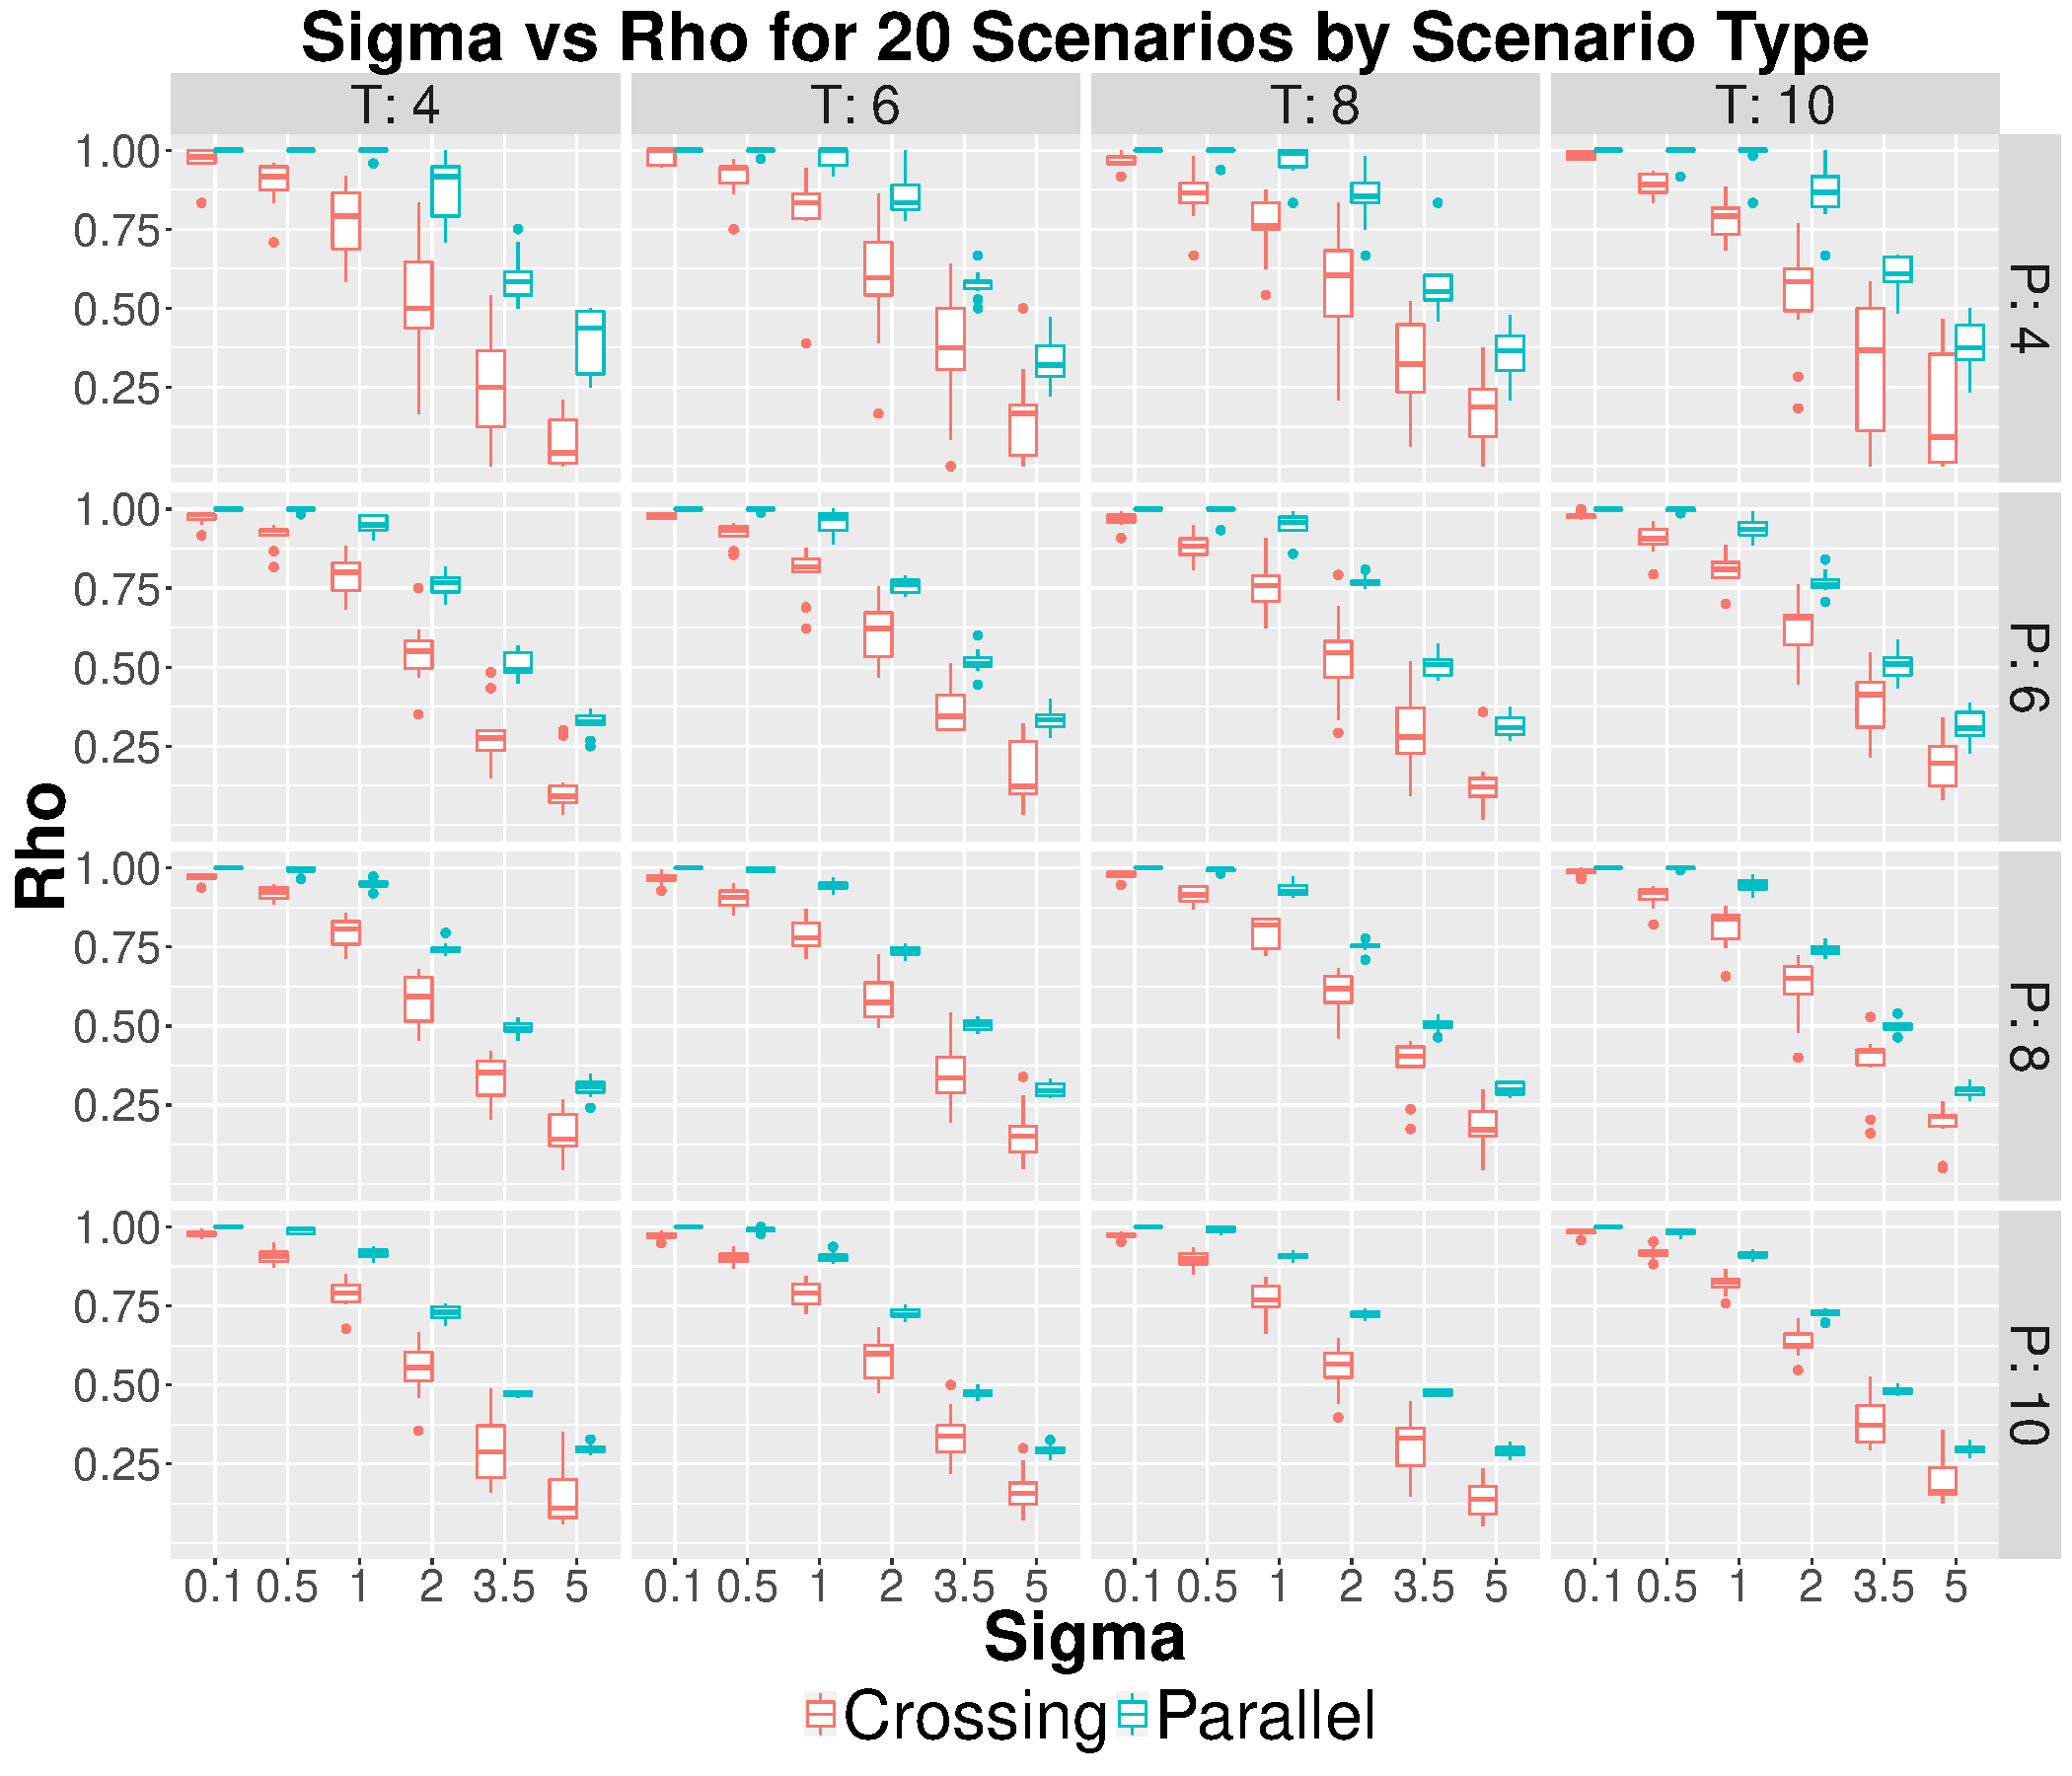
\includegraphics[width=9cm, height=7cm]{Sigma_vs_Rho}
  \caption{Relationship between $\sigma$ and $\rho$ summarized by scenario type for all 20 generated scenarios in this experiment.}
  \label{fig:Sigma_vs_Rho}
\end{figure}

It can be seen that the parallel method of scenario generation on the average creates easier scenarios for the data association problem, as measured by $\rho$,. This result supports the hypothesis that crossing scenarios would be more likely to exhibit detections within close proximity, and consequently result in more difficult scenarios as it pertains to the data association problem. 

In addition, we see from this plot that a relatively small range of six values of $\sigma$ corresponds to the full range of $\rho$ from 0 to 1, meaning that we can quantify data association performance across a more continuous range. This means that $\sigma$ can be used in its natural domain of the data generation process, and $\rho$ can be back calculated as a measurement of difficulty for the data association problem. As a result, we gain a highly interpretable performance metric for the data association problem without sacrificing the ability to generate scenarios in their natural domain. 

\subsubsection{Basic Heuristic}
We begin our discussion of the heuristic with an examination of the run times from the experiment. Table~\ref{tab:Basic_heuristic_times} summarizes the minimum, mean, and maximum run times of the heuristic from this experiment for a single starting point, arranged by the number of targets ($P$) and number of scans ($T$). Times are shown in milliseconds. 

\begin{table}[ht]
\centering
\begin{tabular}{cc|ccc}
  \hline
   & & \multicolumn{3}{c}{Heuristic Run Times } \\
   & & \multicolumn{3}{c}{(in milliseconds)}\\
   P & T & Min & Mean & Max \\ 
  \hline
  \hline
   4 & 4 & 0.07 & 0.10 & 0.18 \\ 
   4 & 6 & 0.18 & 0.24 & 0.38 \\ 
   4 & 8 & 0.34 & 0.45 & 0.62 \\ 
   4 & 10 & 0.58 & 0.76 & 1.02 \\ 
   6 & 4 & 0.11 & 0.15 & 0.25 \\ 
   6 & 6 & 0.31 & 0.39 & 0.58 \\ 
   6 & 8 & 0.64 & 0.81 & 1.05 \\ 
   6 & 10 & 1.24 & 1.56 & 2.02 \\ 
   8 & 4 & 0.14 & 0.19 & 0.30 \\ 
   8 & 6 & 0.46 & 0.57 & 0.86 \\ 
   8 & 8 & 0.95 & 1.24 & 1.58 \\ 
   8 & 10 & 2.07 & 2.53 & 3.37 \\ 
   10 & 4 & 0.19 & 0.25 & 0.41 \\ 
   10 & 6 & 0.63 & 0.80 & 1.03 \\ 
   10 & 8 & 1.44 & 1.84 & 2.44 \\ 
   10 & 10 & 2.96 & 3.73 & 4.56 \\ 
   \hline
\end{tabular}
\caption{Heuristic run times (in milliseconds) for a single starting point.}
\label{tab:Basic_heuristic_times}
\end{table}

Notice that the number of scans has a much greater effect on run times than the number of targets. Whereas the average run time roughly doubles with each increase of 2 scans, the average run time increases as little as 27\% but no more than 50\% for each increase of 2 targets. Therefore, the heuristic scales much more efficiently with $P$ than $T$. Although this may initially seem like a cause for concern, this is actually a desirable trait because it suggests that the heuristic is likely a good candidate for use in a sliding window algorithm. Rather than solve all scans in a single batch at once, a sliding window algorithm solves a subset of scans, or a smaller window, and advances through all scans sequentially.  As the window progresses forward through the scans, "soft" decisions are made meaning that the heuristic would begin with the decisions from the previous solution. As scans pass beyond the horizon and out of the sliding window, the decisions become fixed and we refer to them as "hard" decisions. This process continues until all scans have been processed. The run times of a sliding window variant of the heuristic would not exhibit the curse of dimensionality in $T$ since the number of scans remains constant. Additionally, the heuristic is likely to produce higher quality solutions as a result of these "soft" decisions of previous steps since it is starting from a solution which is likely to be better than a completely random solution. 


Furthermore, the heuristic is extremely parallelizable. This means that we can run different sets of starting points for the heuristic on several computers, allowing either a reduction in total run time for a fixed number of starting points or an increase in the number of starting points for a fixed run time. For example, the average run time for a single starting point of a scenario of six targets and six scans is about 0.4 milliseconds. If we desire to evaluate 50,000 heuristic starting points, we would require about 20 seconds of run time if run in sequence. However, the same number of starting points parallelized onto 100 processors would reduce the total run time to approximately 0.2 seconds. Thus, the run time of the heuristic can be reduced to meet the efficiency needs of the system subject only to the limitation of available processors. 

We continue our evaluation of the basic heuristic by analyzing the performance of its solution on the MIO objective. This gives insight into whether or not the use of RSS as a proxy for the MIO objective is effective. To evaluate effectiveness on these terms, we compute the corresponding MIO objective value of the heuristic solution and normalize it against the MIO objective value of the \textit{ideal} solution, which refers to the solution in which the data association problem is exactly correct (all detection assignments are exactly known). The resulting normalized value represents the MIO objective value as a factor of the ideal solution's MIO objective value. This metric is plotted against $\sigma$ and summarized in Figure~\ref{fig:Basic_Heuristic_Objective}. 

\begin{figure}[h]
  \centering
  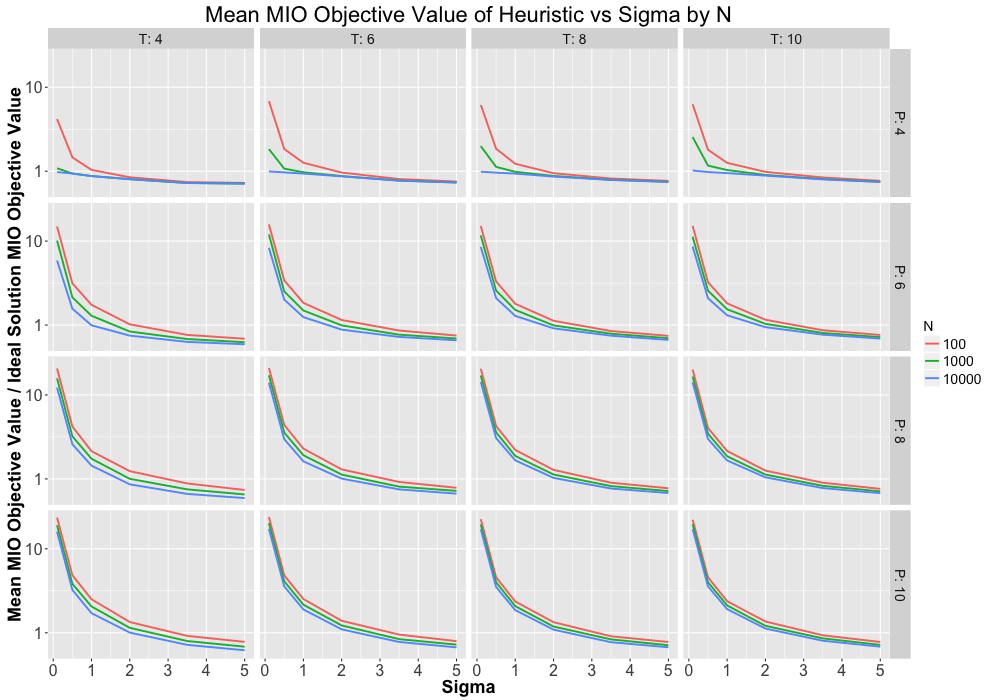
\includegraphics[width=9cm, height=7cm]{Basic_Heuristic_Objective}
  \caption{Heuristic performance as a factor of the ideal solution's MIO objective value.}
  \label{fig:Basic_Heuristic_Objective}
\end{figure}

We see that increasing the number of starting points improves the quality of the heuristic solution as compared to the ideal solution's MIO objective value, especially when the number of targets is small. However, this effect is diminished as the number of targets increases. In addition, we see that for larger numbers of targets, even the largest number of starting points does not achieve near ideal performance, suggesting the need for a much larger number of starting points. This is not considered to be a problem, however, due to the advantages of parallelization discussed previously and also due to the power of optimization, which we will see later. 

We also see that for larger values of $\sigma$ the heuristic actually outperforms the ideal solution's MIO objective value. Remember that the ideal solution is simply ideal in the sphere of data association, while the MIO objective intends to score both the data association and trajectory estimation simultaneously. Therefore, we draw the conclusion that achieving perfect data association for large values of sigma does not necessarily correspond to the best solution to the trajectory estimation problem. In other words, as $\sigma$ increases it may be necessary to tradeoff correct data associations in order to improve the trajectory estimation. We believe the results of the heuristic could be explained by this effect.

Next, we evaluate the performance of the basic heuristic on the data association problem as a function of the number of starting points. To this end, we relationship between accuracy and $N$. Figure~\ref{fig:Basic_Heuristic_Accuracy} plots the mean accuracy of each of the three starting points from this experiment against $\rho$. 

\begin{figure}[h]
  \centering
  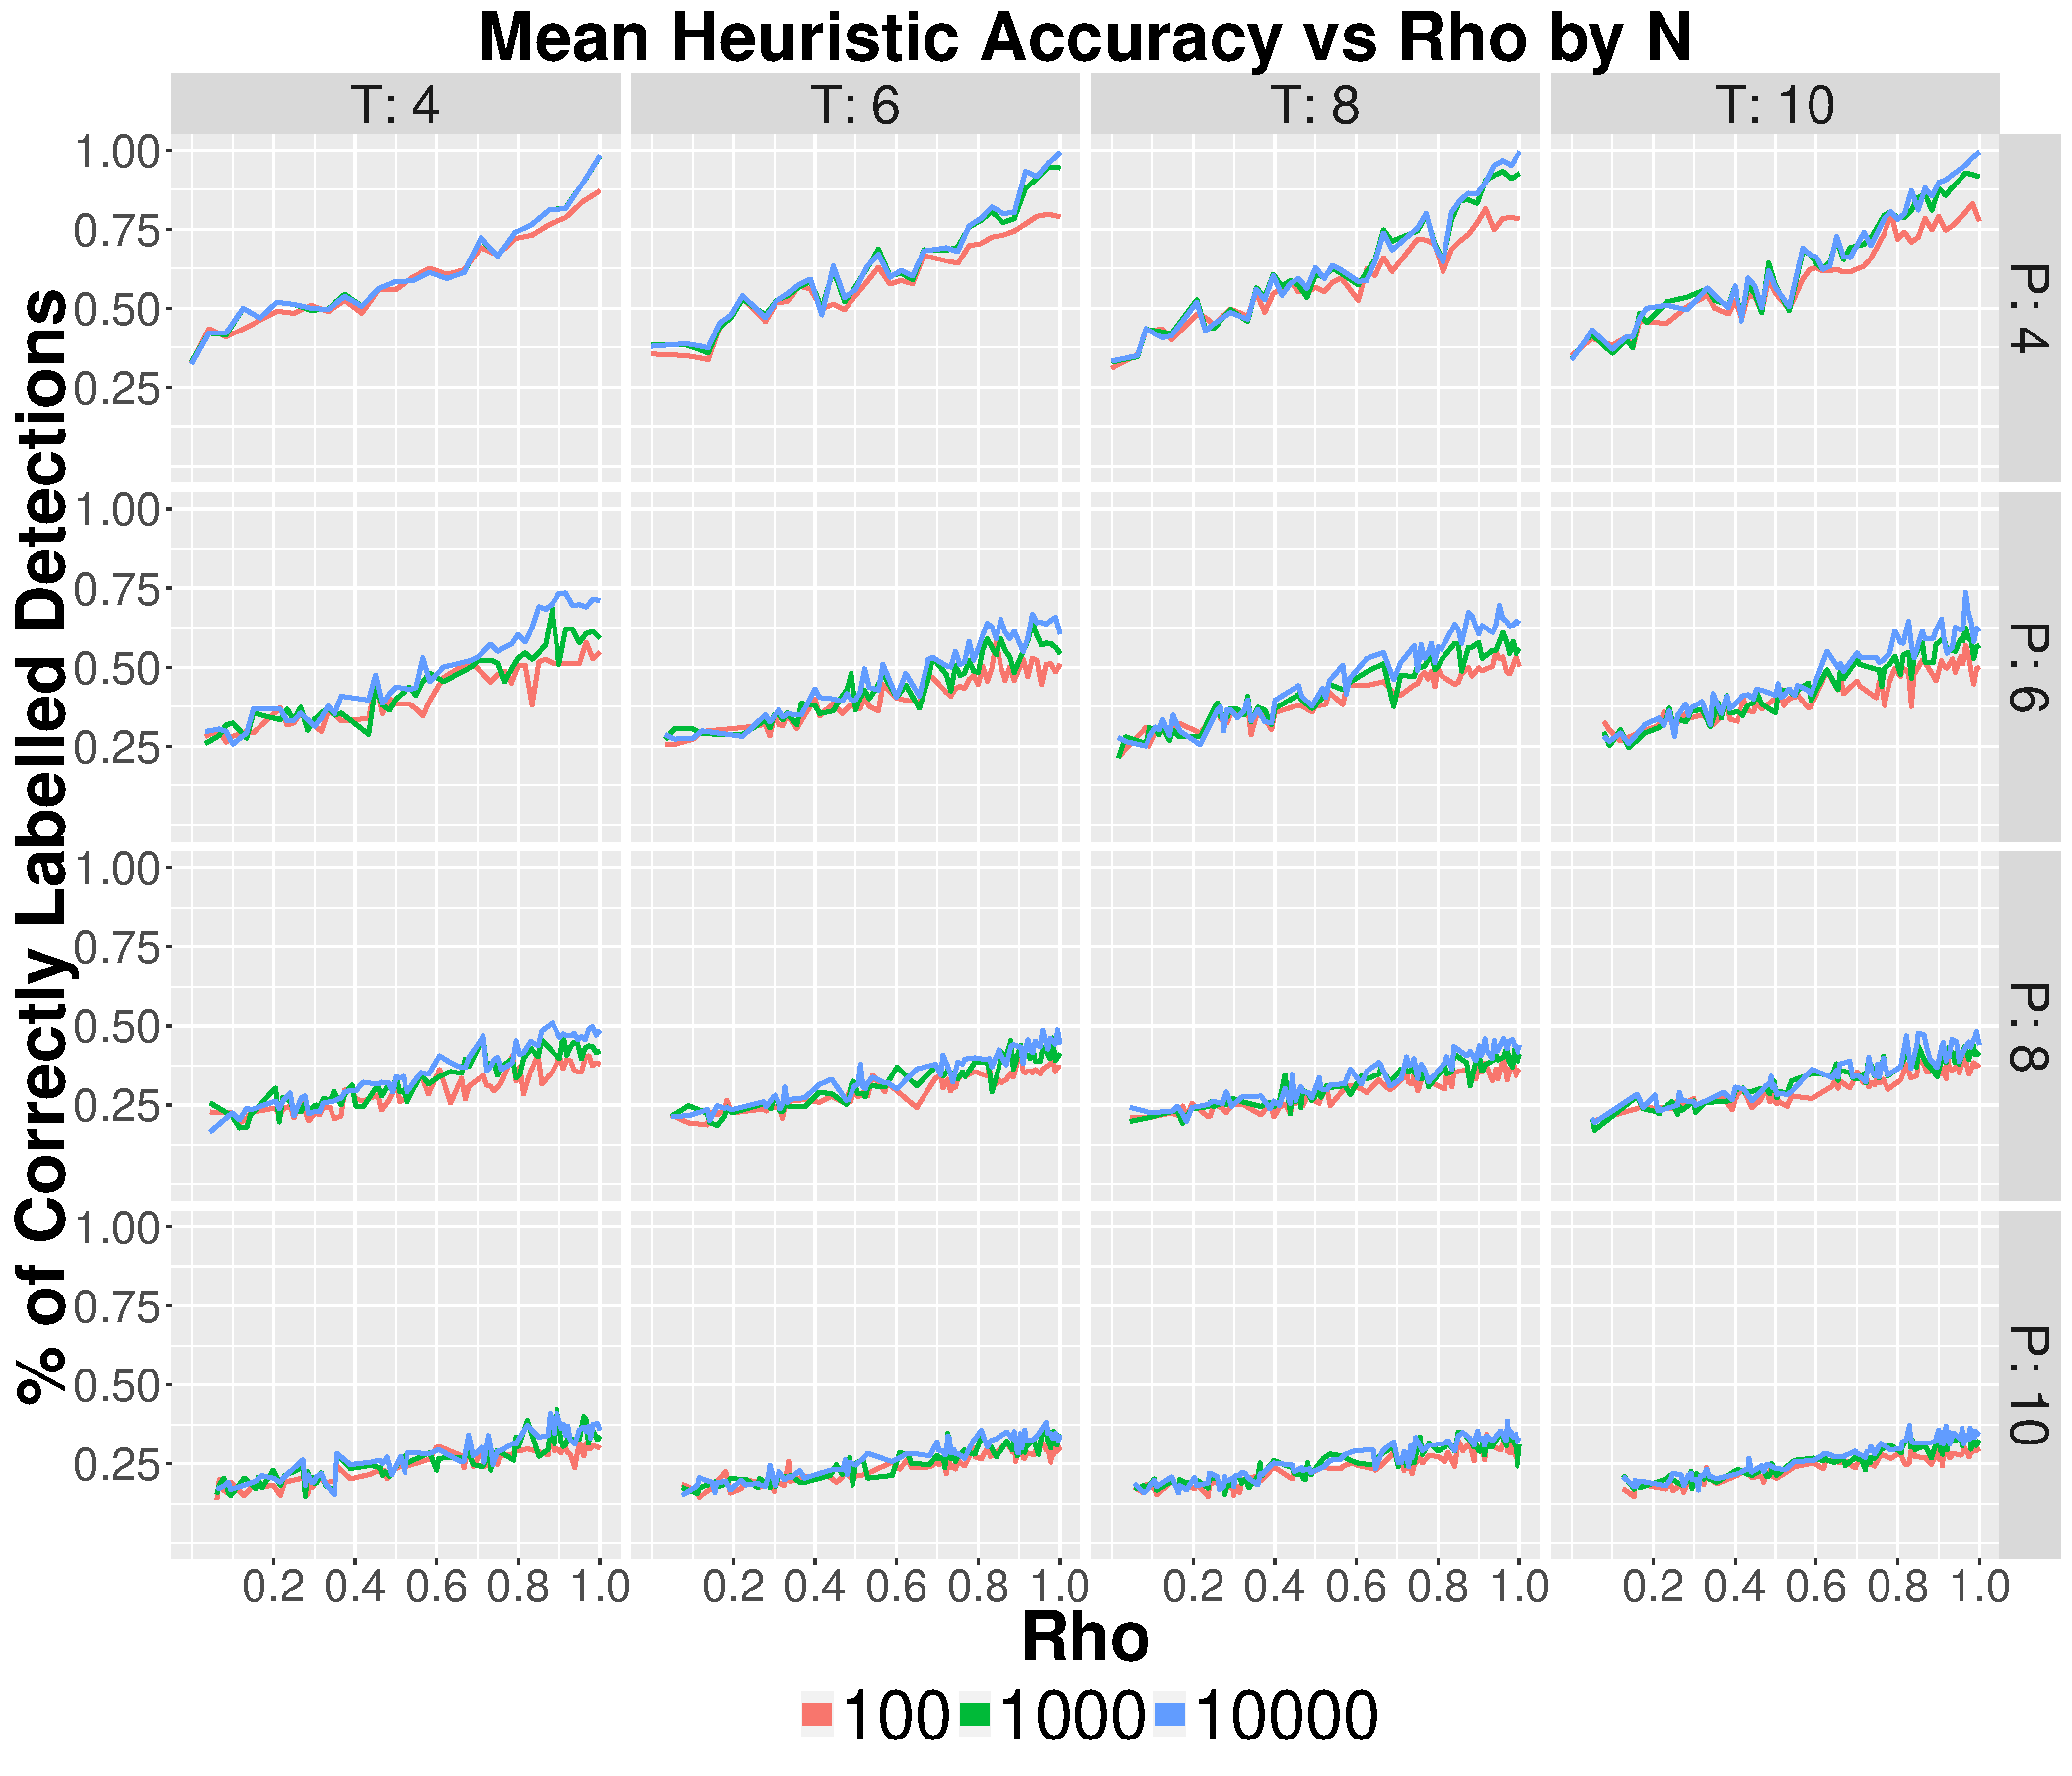
\includegraphics[width=9cm, height=7cm]{Basic_Heuristic_Accuracy}
  \caption{Accuracy of basic heuristic by number of heuristic starting points.}
  \label{fig:Basic_Heuristic_Accuracy}
\end{figure}

First of all, we see that the heuristic finds good solutions to the data association problem, especially for scenarios with fewer targets, but performance degrades as the number of targets increases which is expected. Again it is seen that increasing the number of starting points results in minor improvements, and this improvement is greatest for scenarios with fewer targets. We see a similar effect as $\rho$ increases. We conclude that even small values of $N$ produce moderately good solutions as measured by accuracy.

Overall we conclude that there is not a significant difference in heuristic performance for the range of $N$ values that we explored. Therefore for simplification as we move forward in our analysis, we will restrict our discussions of the heuristic to $N=1,000$.

\subsubsection{Basic MIO}
Next, we transition our evaluation to focus on the MIO by first measuring its performance on the data association problem. Figure~\ref{fig:Basic_Accuracy_Summary} plots the mean accuracy of the MIO, initialized by the $N=1,000$ heuristic solutions, after 1,T, and 2T seconds against $\rho$. We have excluded the data for the MIO after 3T seconds for the sake of clarity as it showed little to no improvement over the MIO after 2T solution. For comparison, we have included the heuristic (for $N=1,000$ only) in addition to a randomized solution, one in which we randomly assigned detections to targets. Note that in this case, that the ideal solution, one in which the associations are exactly correct, achieves an accuracy of 1.0 in all cases so it is not shown explicitly.

\begin{figure}[h]
  \centering  
  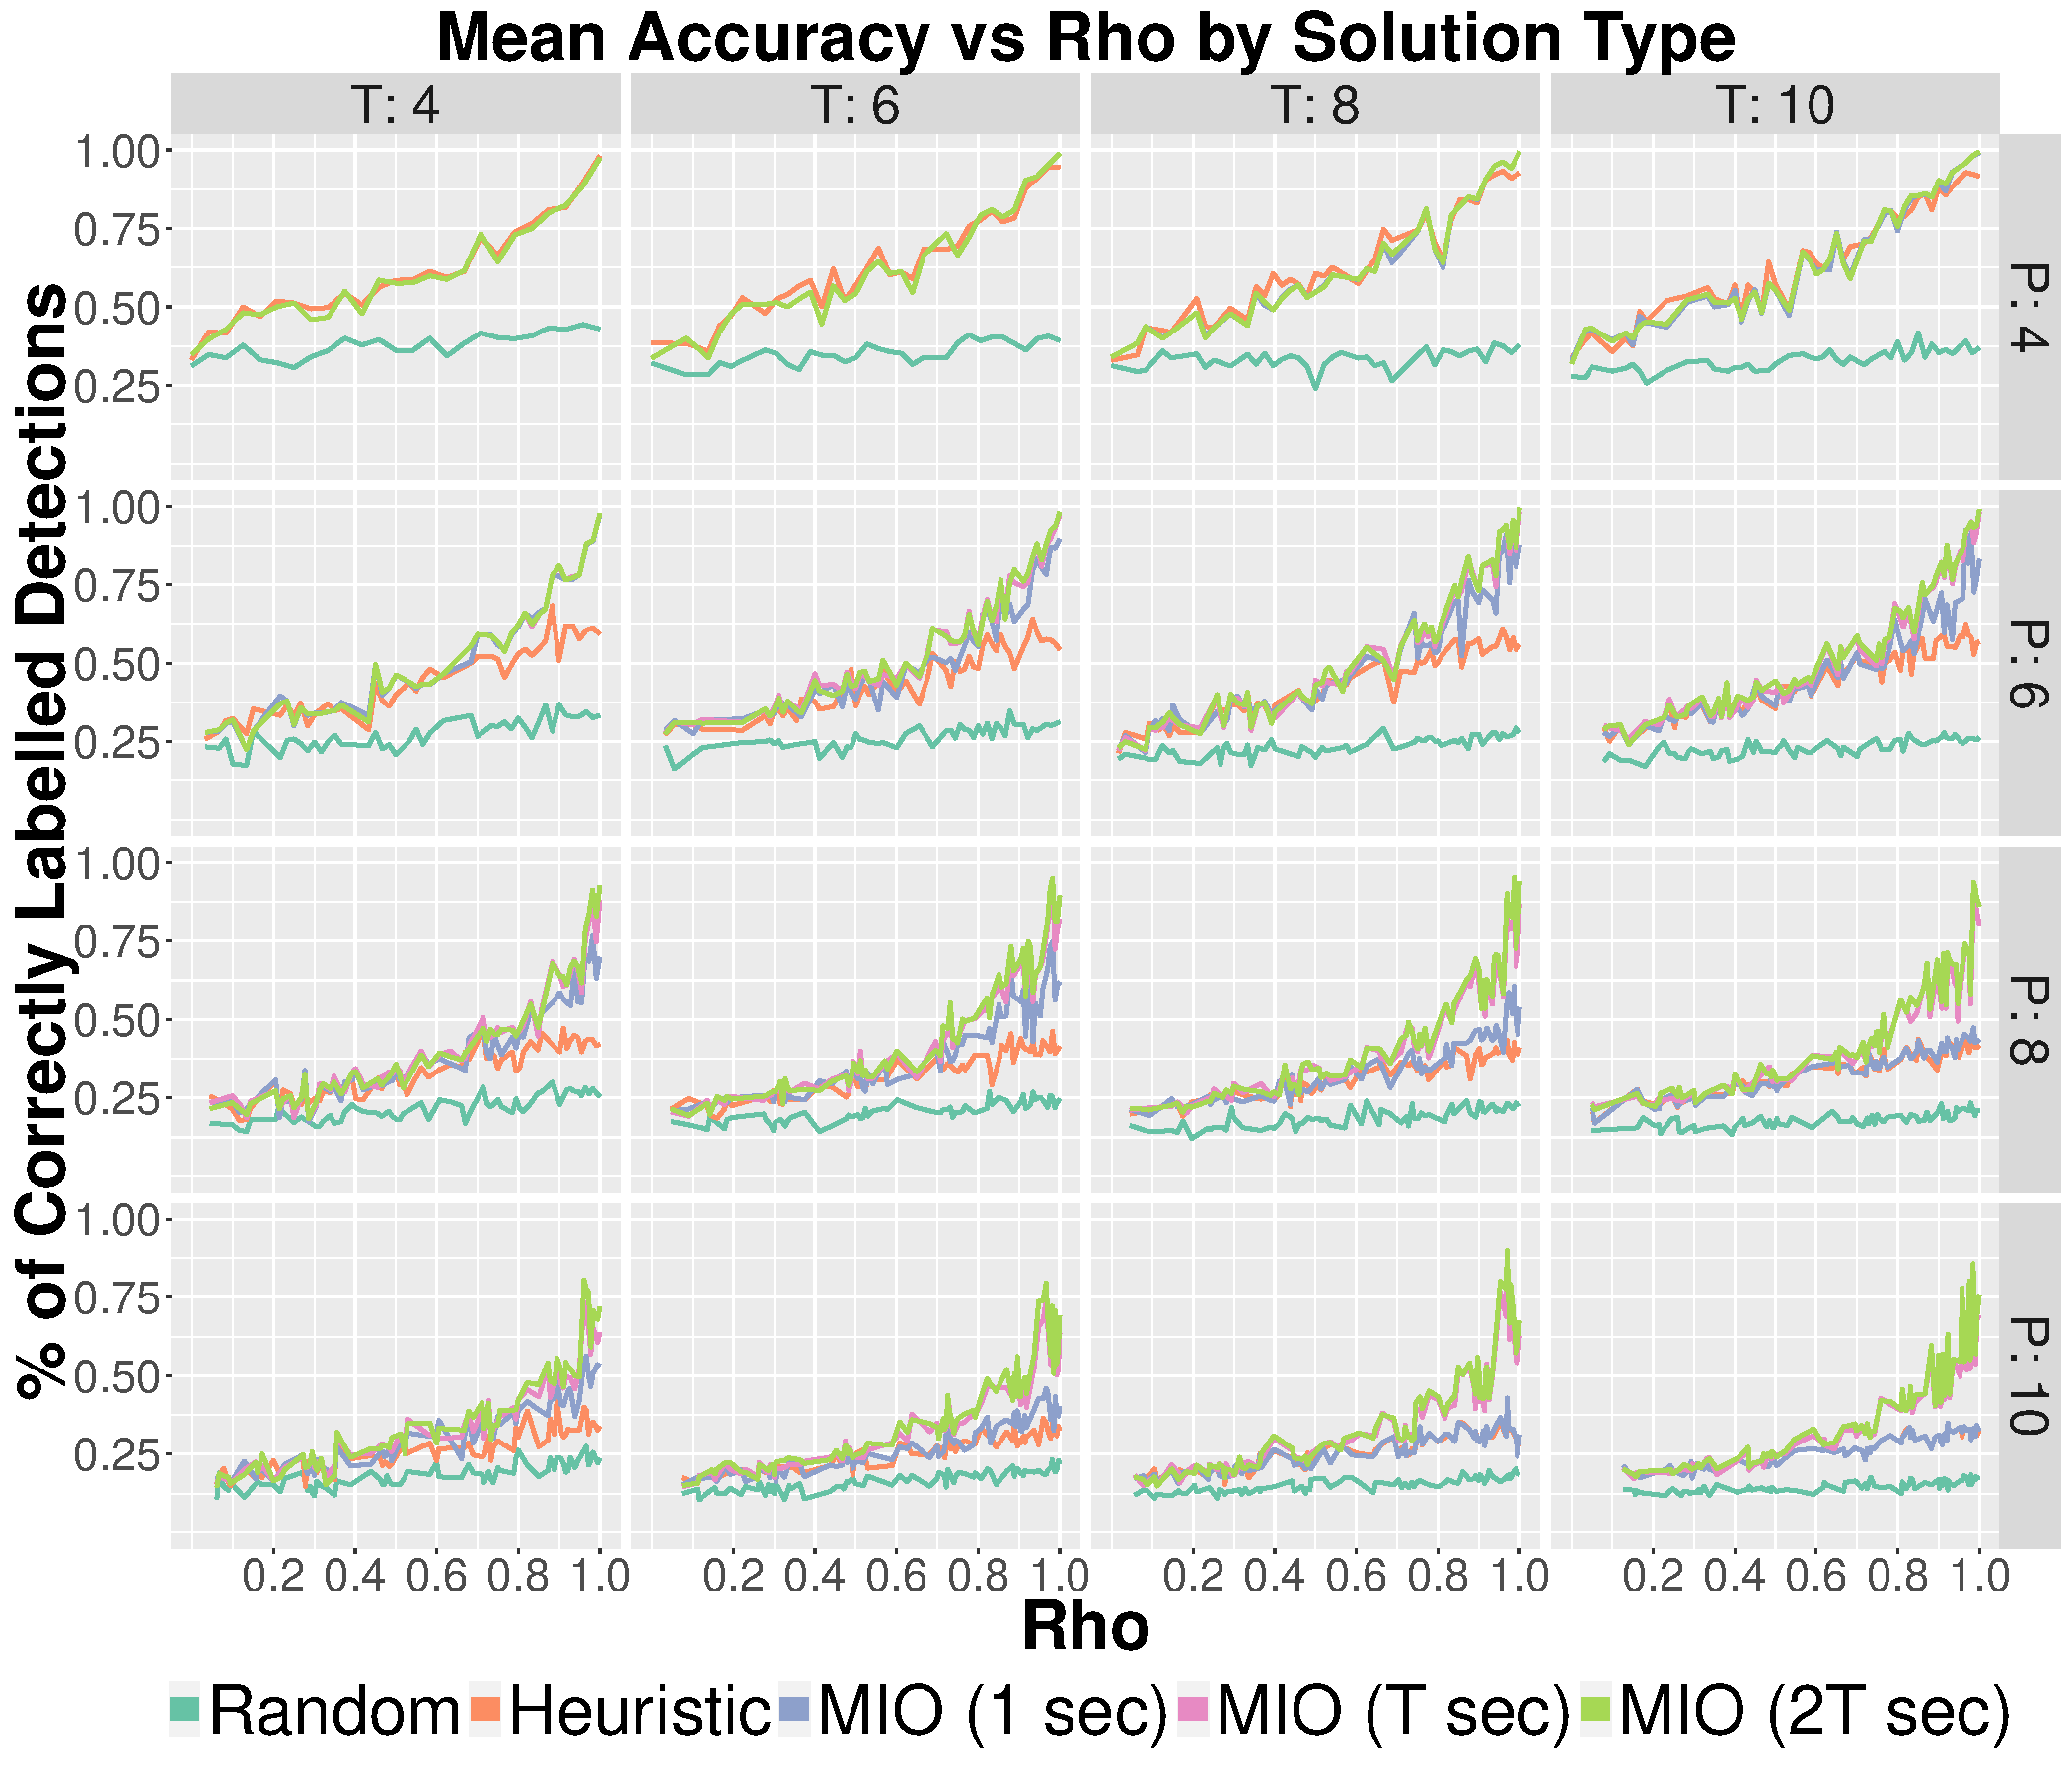
\includegraphics[width=9cm, height=7cm]{Basic_Accuracy_Summary}
  \caption{Accuracy of MIO compared against the heuristic and a randomized solution.}
  \label{fig:Basic_Accuracy_Summary}
\end{figure}

For scenarios with fewer numbers of targets, the MIO solutions were actually proven to be the optimal solution. Therefore, for smaller scenarios with few targets, we see that the heuristic achieves optimal and near optimal solutions. We also see that the easier the scenario, the more improvement the MIO has over the heuristic, while in more difficult scenarios the effect is diminished. Furthermore, it can be seen that in nearly all scenarios, the MIO achieves its best or near best solutions after $T$ or fewer seconds, suggesting the usefulness of the MIO as an online algorithm with a sliding window. 

As mentioned previously in regards to the heuristic, a sliding window algorithm would make decisions on a subset of scans, and these decisions will be fixed before accepting a new set of scans. In regards to the MIO, this would be implemented by adding constraints to restrict the values of $y_{itj}$ to match that of the subsetted solution. The fact that the MIO finds very good solutions in $T$ or fewer seconds means that a sliding window algorithm would be able to solve each subset in real time before advancing to the next subset of scans. Furthermore, the MIO would likely benefit from the fixed decisions of the preceding windows, since this is added knowledge that has not utilized by our approaches.

Next, we evaluate the performance of the basic heuristic and MIO through the lens of trajectory estimation. As discussed previously, we are interested in comparing $\delta$, our proxy for ground track error, against $\sigma$, our measure of difficulty for trajectory estimation, in order to analyze performance of in the sphere of estimation. Figure~\ref{Fig:Basic_Delta_Summary} plots $\sigma$ against $\delta$ for each of the solution types. In addition to the random solution shown on the previous plot, we also add a comparison to the ideal solution, as previously defined.
\begin{figure}[h]
  \centering
  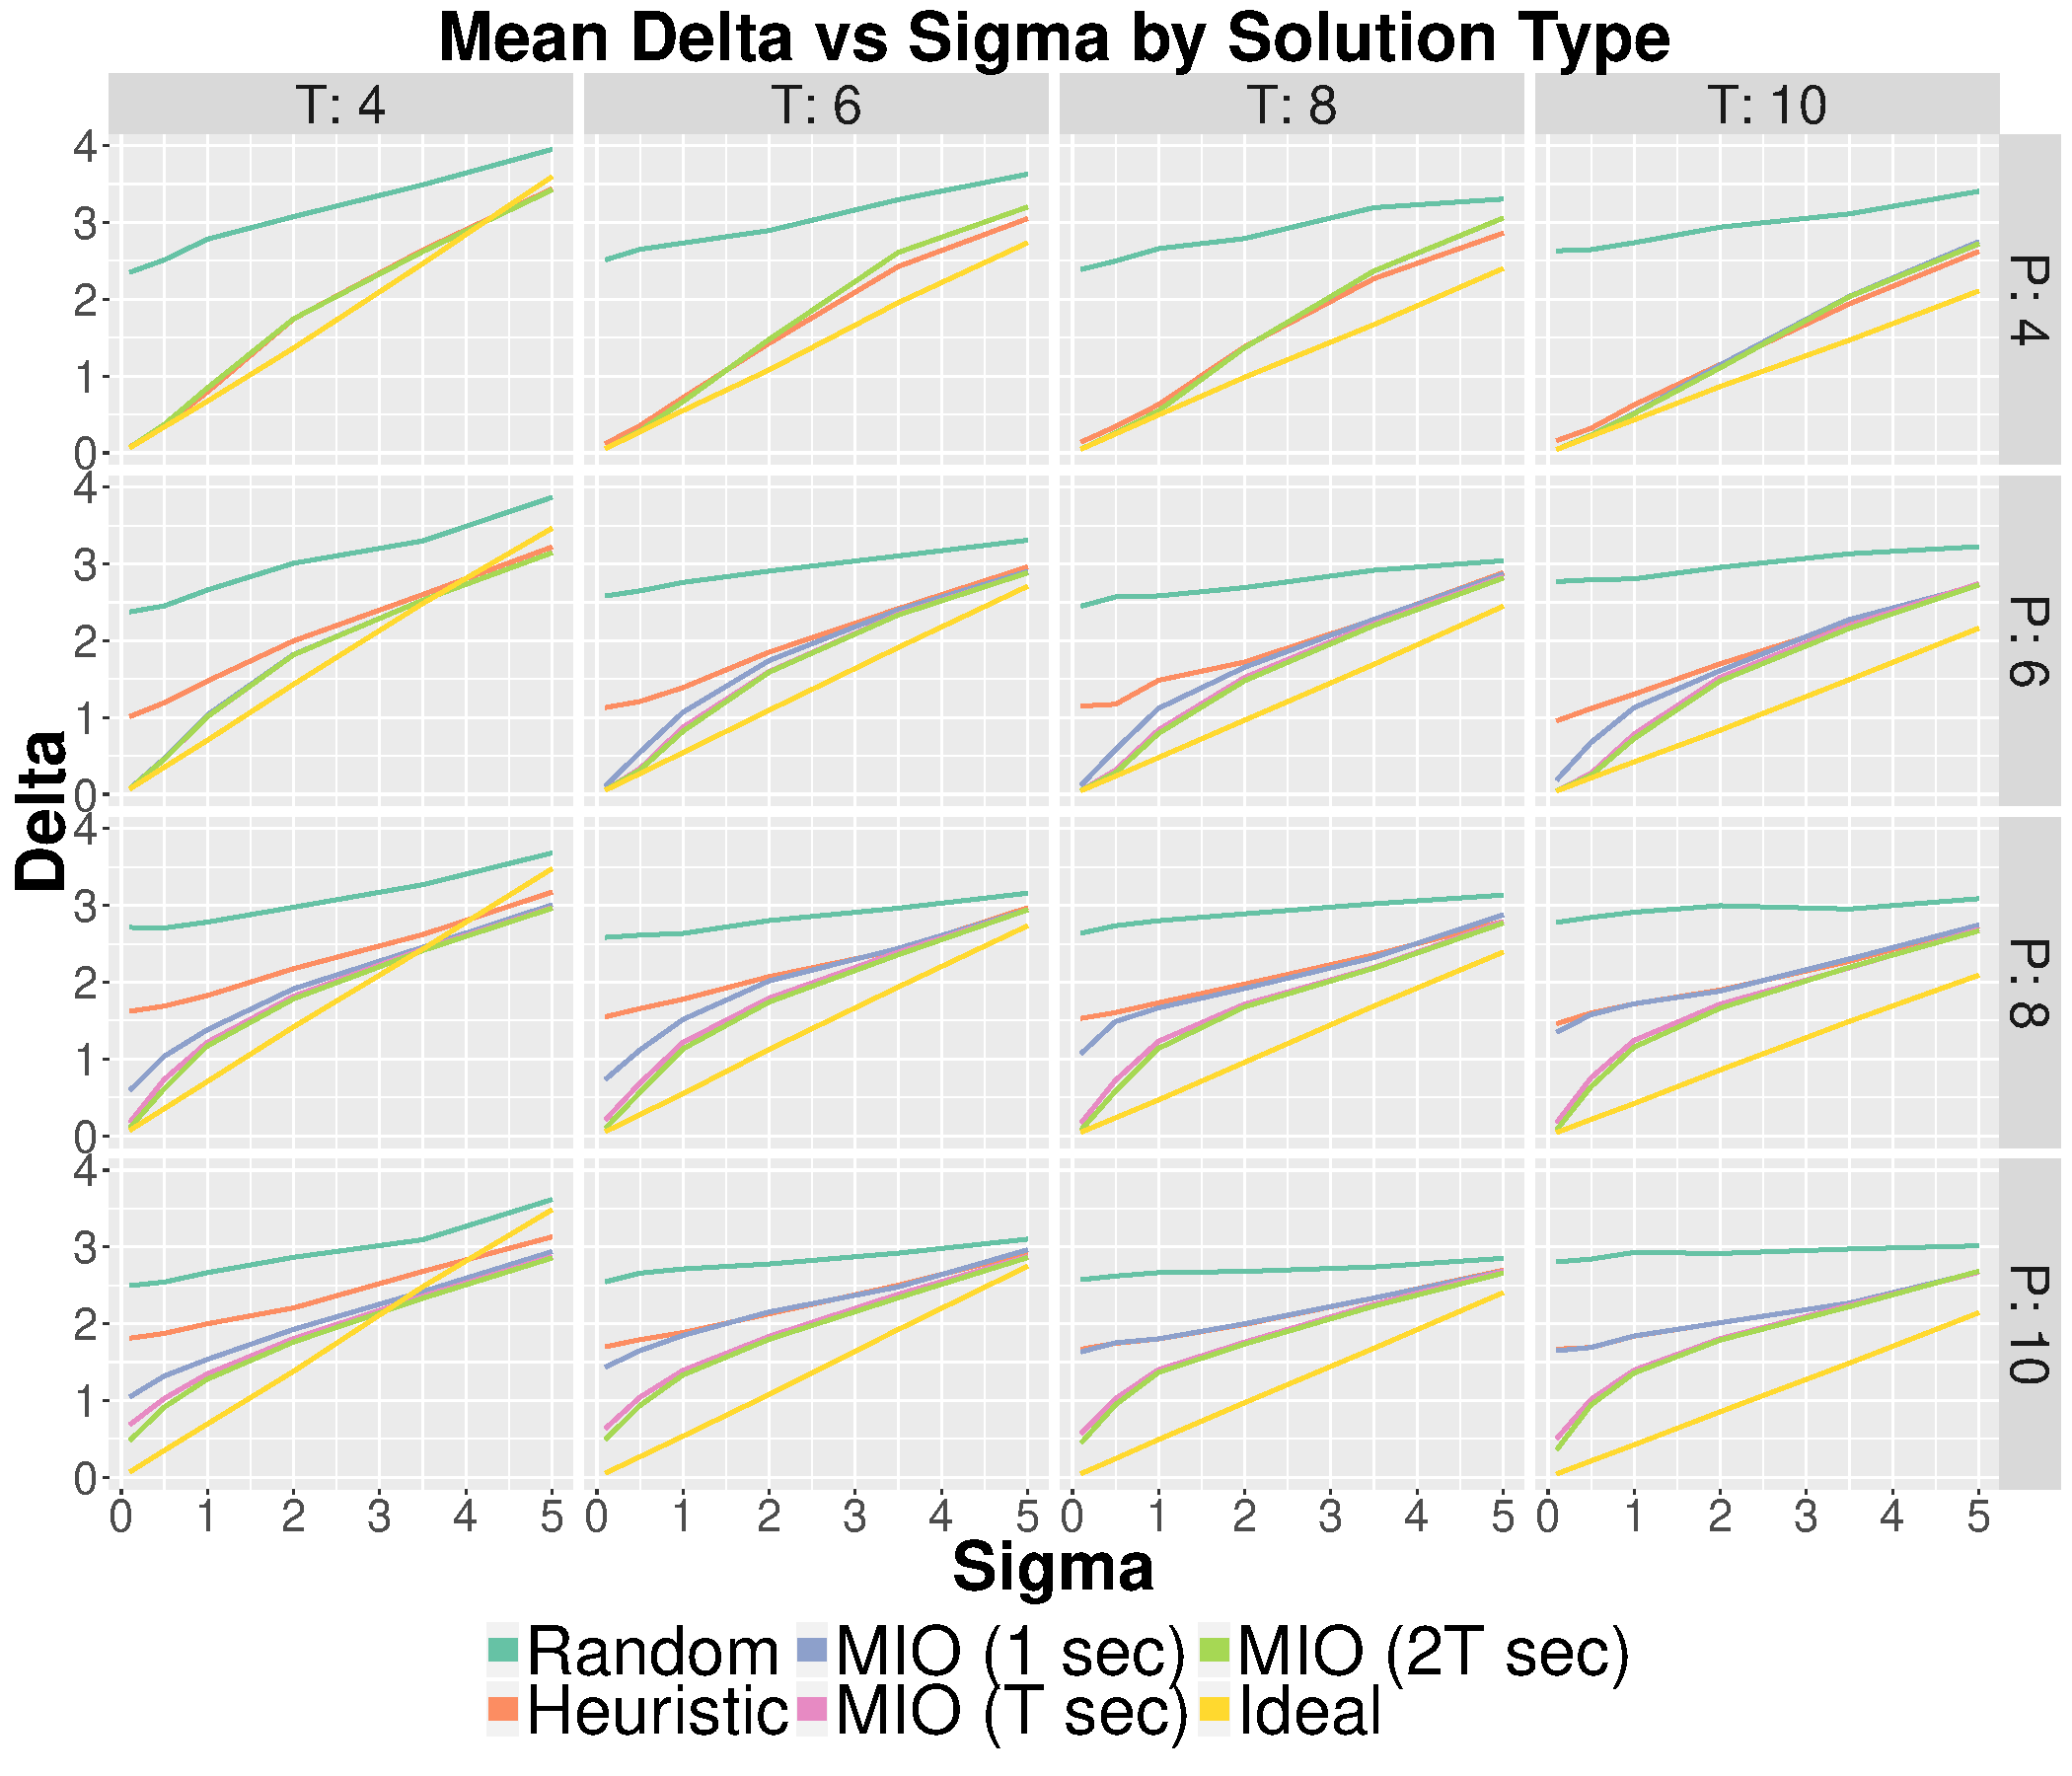
\includegraphics[width=9cm, height=7cm]{Basic_Delta_Summary}
  \caption{Trajectory estimation performance}
  \label{Fig:Basic_Delta_Summary}
\end{figure}

Remember that lower values of delta correspond to trajectory estimations that are closer to that of the true ground track. We see that the performance of the heuristic converges to that of the MIO for scenarios with few targets, as well as for large values of $\sigma$. Additionally, we see that as the number of targets increases we begin to see stronger improvements by the MIO over the heuristic. Interestingly, we see that for the scenarios with the largest number of targets and scans, the MIO after one second is not much better than the heuristic. While the MIO after T seconds provides significant improvement over that of the heuristic and MIO after 1 second, there is little further improvement in running the MIO for 2T seconds. 

Again, we see that in scenarios with only for scans ($T=4$) we see that for larger values of $\sigma$ the heuristic and/or MIO sometimes outperforms the ideal. This is likely a result of limited data and increases uncertainty under high noise. As the number of scans approaches infinity, the ideal solution, or perfect data associations, leads to trajectory estimates that are closer and closer to the true ground track. Put differently. as more and more data is known, it becomes easier to estimate the trajectories even in the event of large noise, and so the trajectory estimates that result from the ideal solution converges to the true ground track. 

\subsection{Robust Experimental Simulations \& Computational Results}\label{sec:Robust_Results}
Here we extend the discussion from the previous section to analyze the performance of our methods on scenarios with detection ambiguity. We first summarize our experimental methods before discussing performance of both the robust heuristic and the robust MIO in the spheres of both the data association and trajectory estimation problems.

This experiment serves as an extension of the basic one, in order to test the performance of our algorithms under detection ambiguity. We use the same scenarios generated from the basic experiment, but due to the additional difficulty inherent with detection ambiguity, we limit the range of signal noise to $\sigma \in \{0.1,0.5,1.0,2.0\}$, excluding choosing to exclude the extreme cases of signal noise. In addition, we simulate both missed detections and false alarms. A detection is removed with probability, $\gamma$, and we consider $\gamma \in \{0.2,0.15,0.1,0.05\}$. We do not allow empty scans. For each scan, we generate false alarms according to a poisson distribution with parameter, $\lambda$, and detection locations are then randomly selected uniformly within the state space. We consider $\lambda \in \{0.1,0.5,0.1,2.0\}$. The false alarms are then added to $\mathcal{X}_{t}$ and the detection order of $\mathcal{X}_{t}$ is again randomly shuffled as before. 

Once the data has been generated, we follow the same sequence as before in the basic experiment, running the heuristic first and then feeding the solution into the MIO as a warm start. Note that the heuristic is given 1,000 starting points only, as concluded from the results of the basic experiment. Once again, the optimization process was set to terminate after 3T seconds, with solutions collected at intervals of $\{1,T,2T,3T\}$ seconds. Prior to the running of this experiment, we performed a mini experiment and used the results to tune the penalties $\theta$ and $\phi$. A summary of the exact penalties used along with an explanation of the insight behind them, can be found in Appendix~\ref{sec:Penalty_Appendix}. 

We will now evaluate the performance of the robust heuristic and MIO. We begin with a discussion on the run times of the robust heuristic, following the number of targets estimation, accuracy and trajectory estimation.

\subsubsection{Robust Heuristic Run Times} Table~\ref{tab:Robust_heuristic_times} summarizes the minimum, mean, and maximum run times of the heuristic from Experiment 2 for a single starting point, arranged by the number of estimate targets ($P_{estimated}$) and number of scans ($T$). Times are shown in milliseconds. 

\begin{table}[ht]
\centering
\begin{tabular}{cc|ccc}
  \hline
   & & \multicolumn{3}{c}{Heuristic Run Times } \\
   & & \multicolumn{3}{c}{(in milliseconds)}\\
   $ P_{\text{estimated}}$ & T & Min & Mean & Max \\ 
  \hline
  \hline
  2 & 4 & 0.15 & 0.23 & 0.41 \\ 
  2 & 6 & 0.42 & 0.56 & 0.93 \\ 
  2 & 8 & 0.77 & 1.04 & 2.24 \\ 
  2 & 10 & 1.27 & 1.73 & 20.23 \\ 
  4 & 4 & 0.15 & 0.34 & 1.04 \\ 
  4 & 6 & 0.50 & 0.94 & 2.69 \\ 
  4 & 8 & 1.09 & 1.88 & 3.87 \\ 
  4 & 10 & 2.12 & 3.25 & 13.51 \\ 
  6 & 4 & 0.14 & 0.42 & 0.96 \\ 
  6 & 6 & 0.57 & 1.29 & 4.45 \\ 
  6 & 8 & 1.33 & 2.66 & 75.28 \\ 
  6 & 10 & 2.53 & 4.61 & 18.69 \\ 
  8 & 4 & 0.16 & 0.50 & 1.10 \\ 
  8 & 6 & 0.60 & 1.59 & 3.46 \\ 
  8 & 8 & 1.38 & 3.37 & 6.87 \\ 
  8 & 10 & 2.63 & 5.84 & 12.40 \\ 
  10 & 4 & 0.18 & 0.55 & 1.10 \\ 
  10 & 6 & 0.72 & 1.82 & 3.98 \\ 
  10 & 8 & 1.53 & 3.96 & 8.18 \\ 
  10 & 10 & 3.42 & 6.93 & 13.93 \\ 
  12 & 4 & 0.16 & 0.56 & 0.99 \\ 
  12 & 6 & 0.99 & 1.95 & 3.96 \\ 
  12 & 8 & 1.74 & 4.33 & 8.69 \\ 
  12 & 10 & 3.40 & 7.71 & 15.10 \\ 
   \hline
\end{tabular}
\caption{Robust heuristic run times (in milliseconds) for a single starting point.}
\label{tab:Robust_heuristic_times}
\end{table}

Comparing Table~\ref{tab:Basic_heuristic_times} and Table~\ref{tab:Robust_heuristic_times} we see that the run times for an estimated number of targets in the robust heuristic range from roughly double to three and four times that of a comparable number of targets in the basic heuristic. Due to the increase in combinatorial solutions in the robust heuristic over the basic heuristic, this was an expected result. The robust heuristic, however, can be parallelized in the same many as the basic heuristic, meaning that the robust heuristic can actually recover the speed of the basic heuristic with the introduction of additional processors. More importantly, we see that the robust heuristic scales very efficiently with $P_{\text{estimated}}$, and this the scaling actually improves as the number of estimated targets and scans increases. Increasing from two to six estimated targets for four scans roughly triples the run time, while increasing from eight to twelve estimated targets for four scans increases the run time by only 12\%. This is a great result because it means that a relatively wide range of estimated targets can be parallelized without fear of one subset requiring a substantially longer run time than another. 

Although the robust heuristic scales well with the number of estimated targets, it is more sensitive to increases in the number of scans. However, this effect is no worse than what we saw for the basic heuristic. It appears that on average increasing the number of scans by 2 results in a doubling of the run time for a fixed number of estimated targets. We conclude that these results again support the use of the robust heuristic in an online algorithm with a sliding window, as discussed in the previous section.
 
\subsubsection{Evaluating the Number of Targets}
Next, we continue our analysis of the robust approaches by quantifying the algorithms' ability to estimate the correct number of targets. This is perhaps the most important goal of a MTT algorithm and so we begin our analysis here. To this end, we define
\begin{align}
	P_{\text{difference}} = P_{\text{true}} - P_{\text{estimated}}
\end{align}

where $P_{\text{estimated}}$ is the number of estimated targets and $ P_{\text{true}}$ is the number of true targets, and we plot the distribution of $P_{\text{estimated}}$. Figure~\ref{fig:Robust_4_8_Histogram} shows the distribution of $P_{\text{difference}}$ for scenarios with four targets and eight scans, and for comparison, Figure~\ref{fig:Robust_8_8_Histogram} plots the same result for scenarios of eight targets and eight time scans. 
\begin{figure}[h]
  \centering
  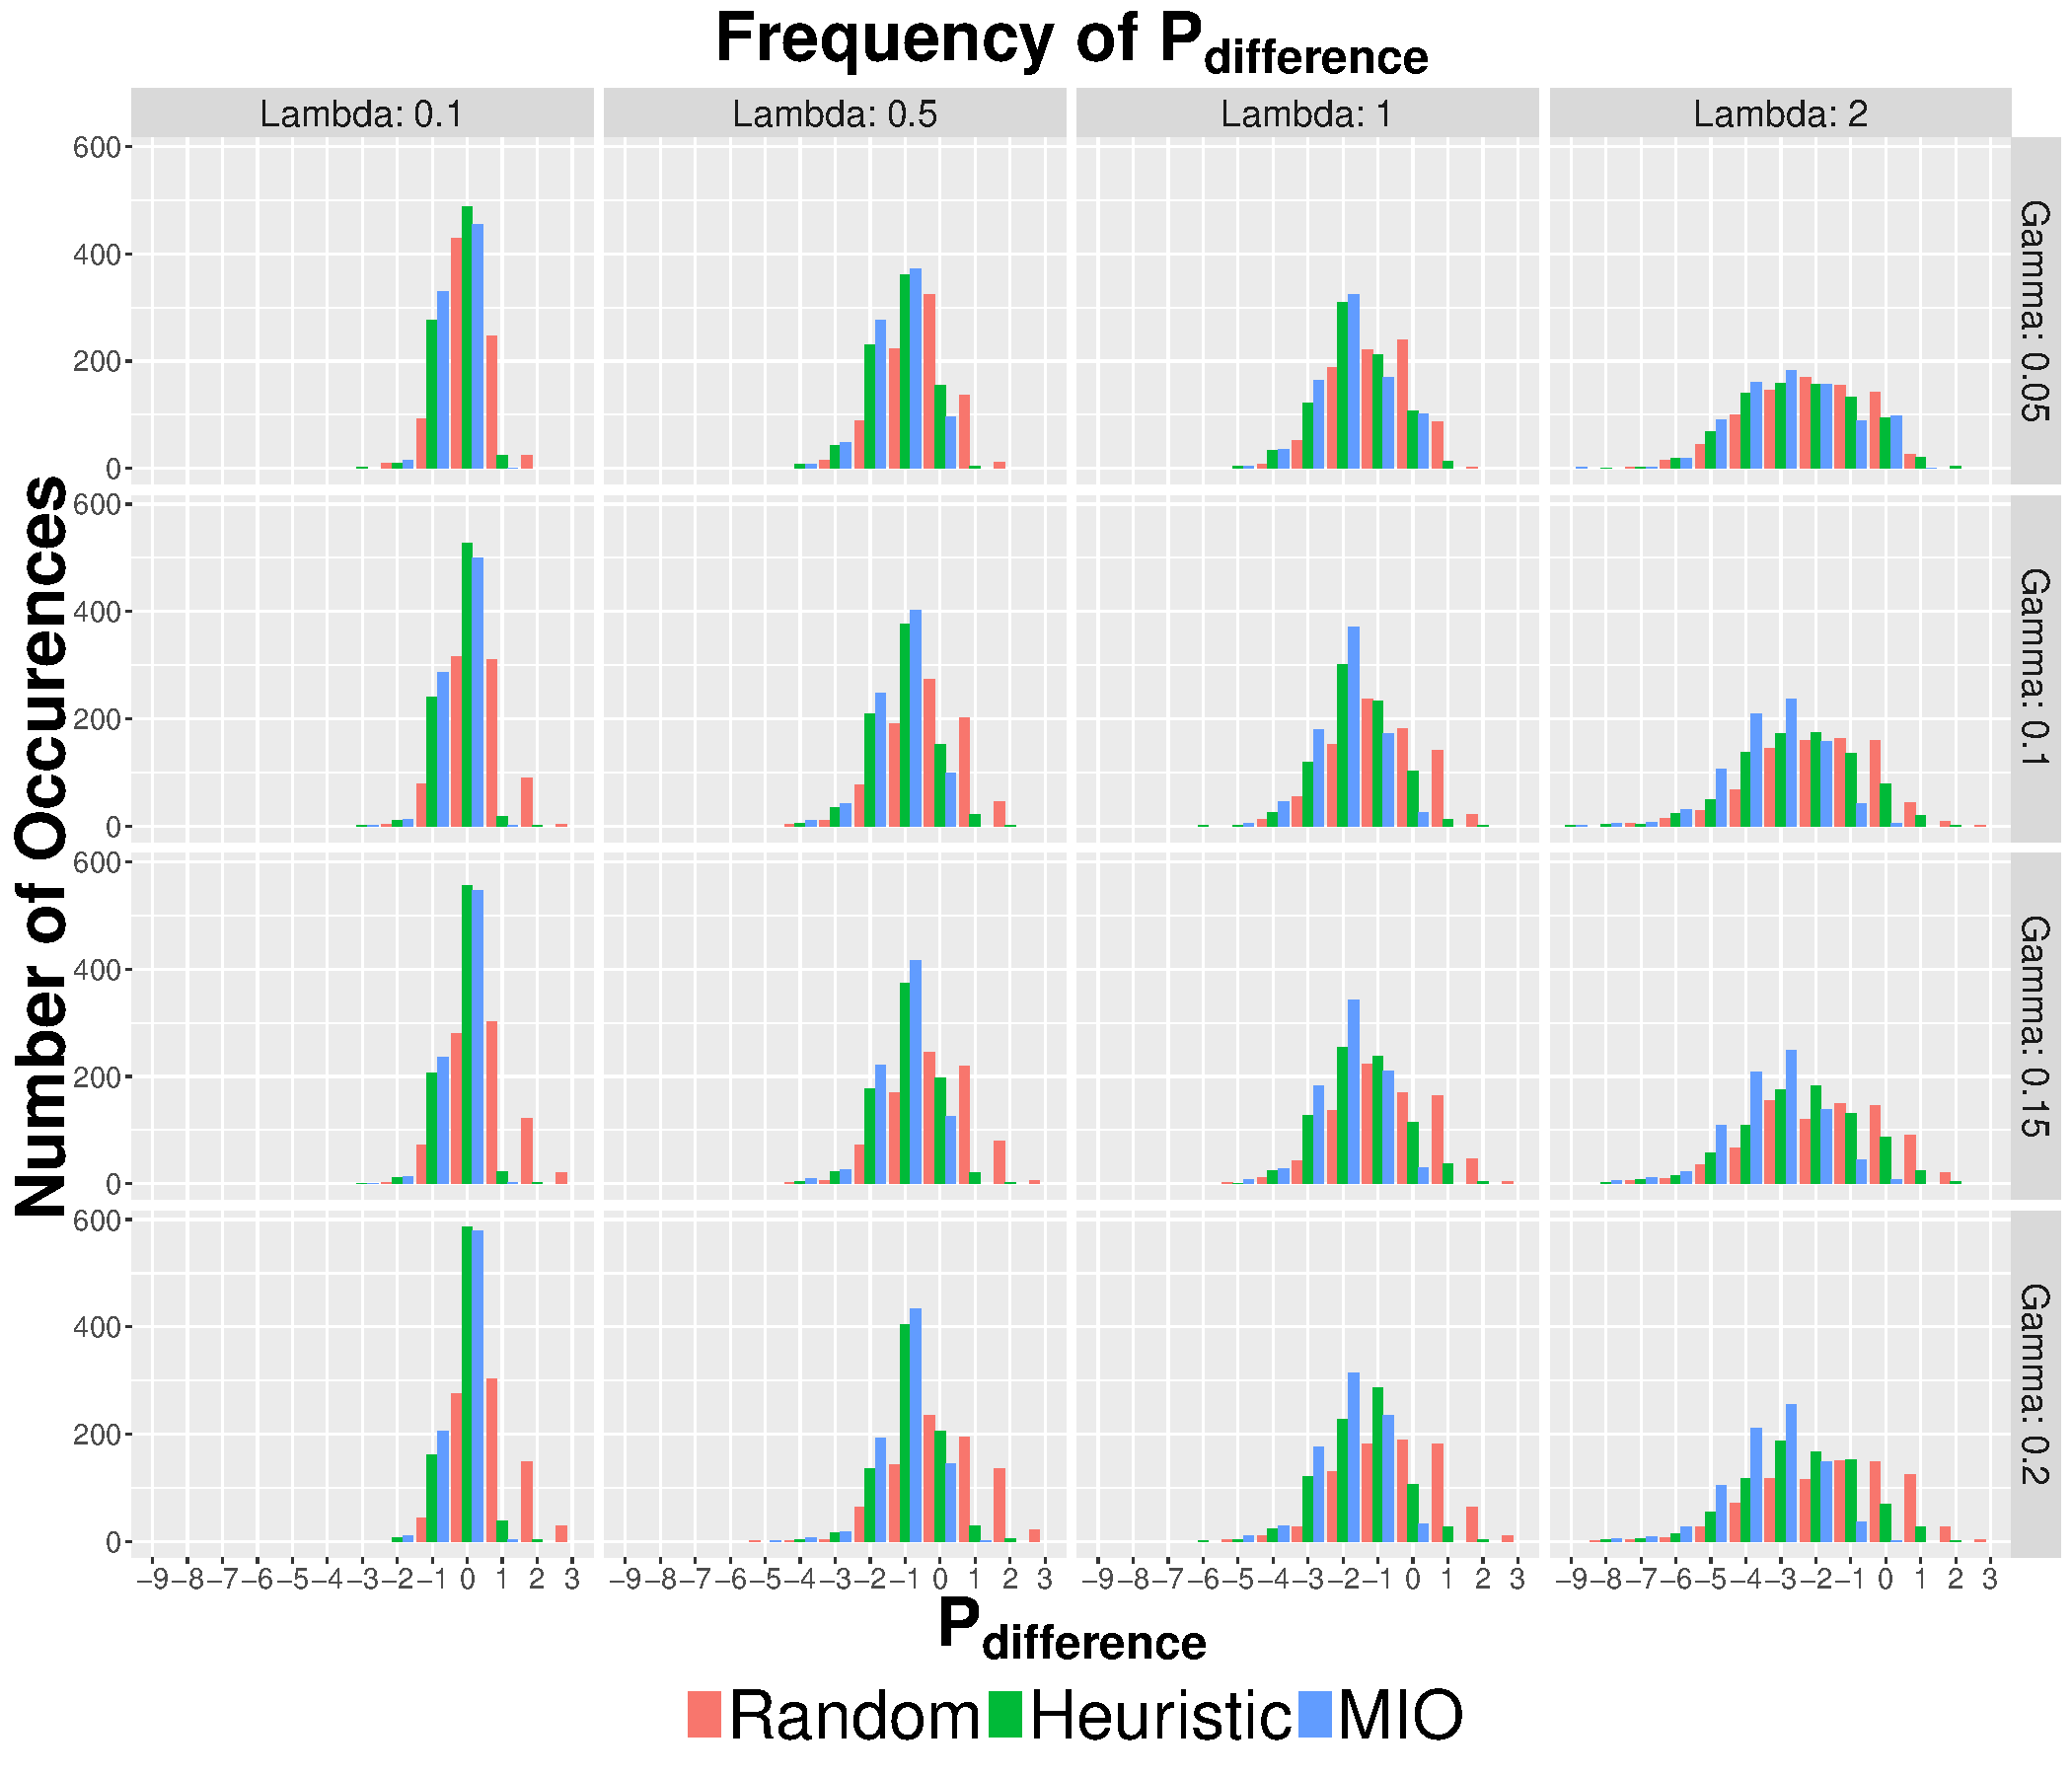
\includegraphics[width=9cm, height=7cm]{4_8_Histogram}
  \caption{Distribution of the difference in true and estimated number of targets for scenarios with 4 targets and 8 scans, arranged by $\gamma$ and $\lambda$.}
  \label{fig:Robust_4_8_Histogram}
\end{figure}

\begin{figure}[h]
  \centering
  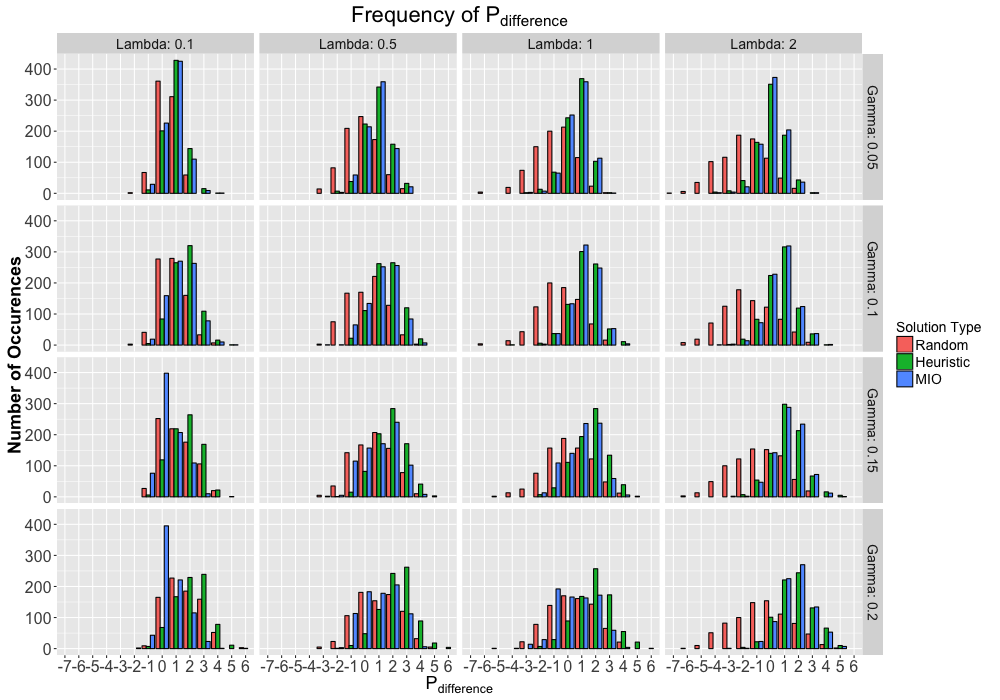
\includegraphics[width=9cm, height=7cm]{8_8_Histogram}
  \caption{Distribution of the difference in true and estimated number of targets for scenarios with 8 targets and 8 scans, arranged by $\gamma$ and $\lambda$.}
  \label{fig:Robust_8_8_Histogram}
\end{figure}

Note that the algorithms have correctly estimated the number of targets when $P_{\text{difference}} = 0$. When $P_{\text{difference}} < 0$, we have overestimated the number of targets, and when $P_{\text{difference}} > 0$, we have underestimated the number of targets. We see that both the robust heuristic and the robust MIO estimate the number of targets correctly a high proportion of the time in the scenario with four targets, particularly for smaller values of $\lambda$. As $\lambda$ increases, though, both algorithms tend to underestimate. The same trend persists in the larger scenario. This suggests that either 1) the false alarm penalty needs further tuning and likely was not set high enough in the experiment or 2) the missed detection penalty set too high. In the case where $\theta$ is set too low, the algorithms would prefer to classify detections as false alarms rather than create additional trajectories for the detections. In the case of $\phi$ set too high, the algorithms would opt out of creating additional trajectories in order to decrease the need to fill smaller scans with missed detections. Furthermore, because the effect of underestimation is more prominent in the scenario with more targets, we conclude that both penalties should probably take into account the number of targets that it is currently estimating.

\subsubsection{Data Association}
Knowing that we tend to underestimate the number of targets with the given penalties, we move on in our analysis to measuring the accuracy of our robust approaches. Figures~\ref{fig:Robust_4_8_Accuracy} and~\ref{fig:Robust_8_8_Accuracy} plot the accuracy performance metric against the difficulty metric, $\rho$, for scenarios of four and eight targets, respectively. Both scenarios have eight scans and both Figures have been arranged by $\gamma$ and $\lambda$.
\begin{figure}[h]
  \centering
  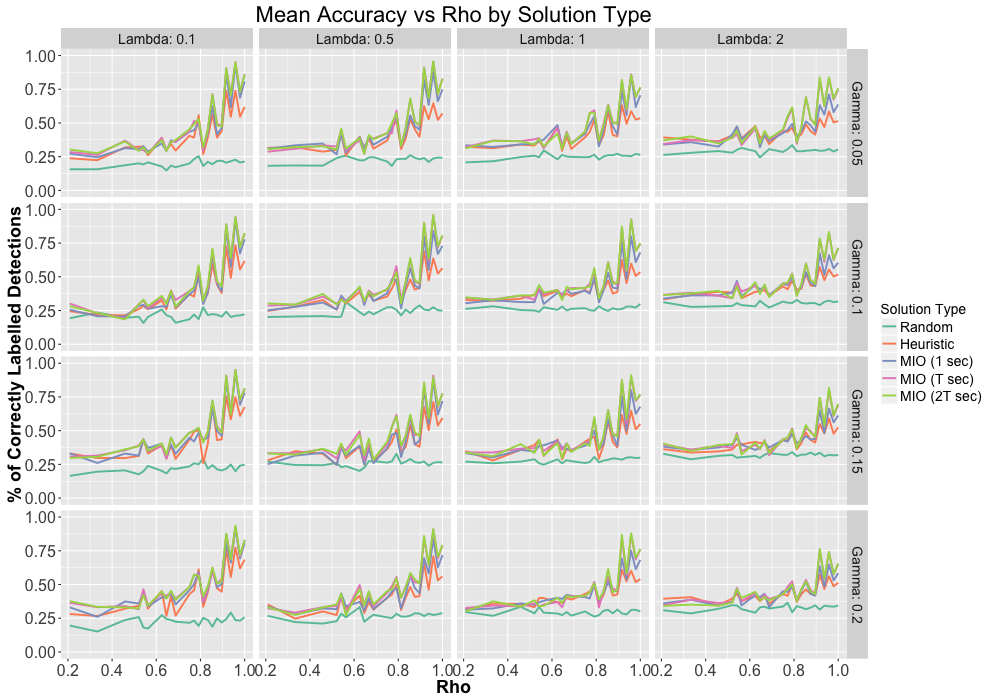
\includegraphics[width=9cm, height=7cm]{4_8_Accuracy}
  \caption{Accuracy of robust heuristic and MIO as compared to random solutions for scenarios of 4 targets and 8 scans, arranged by $\gamma$ and $\lambda$.}
  \label{fig:Robust_4_8_Accuracy}
\end{figure}

\begin{figure}[h]
  \centering
  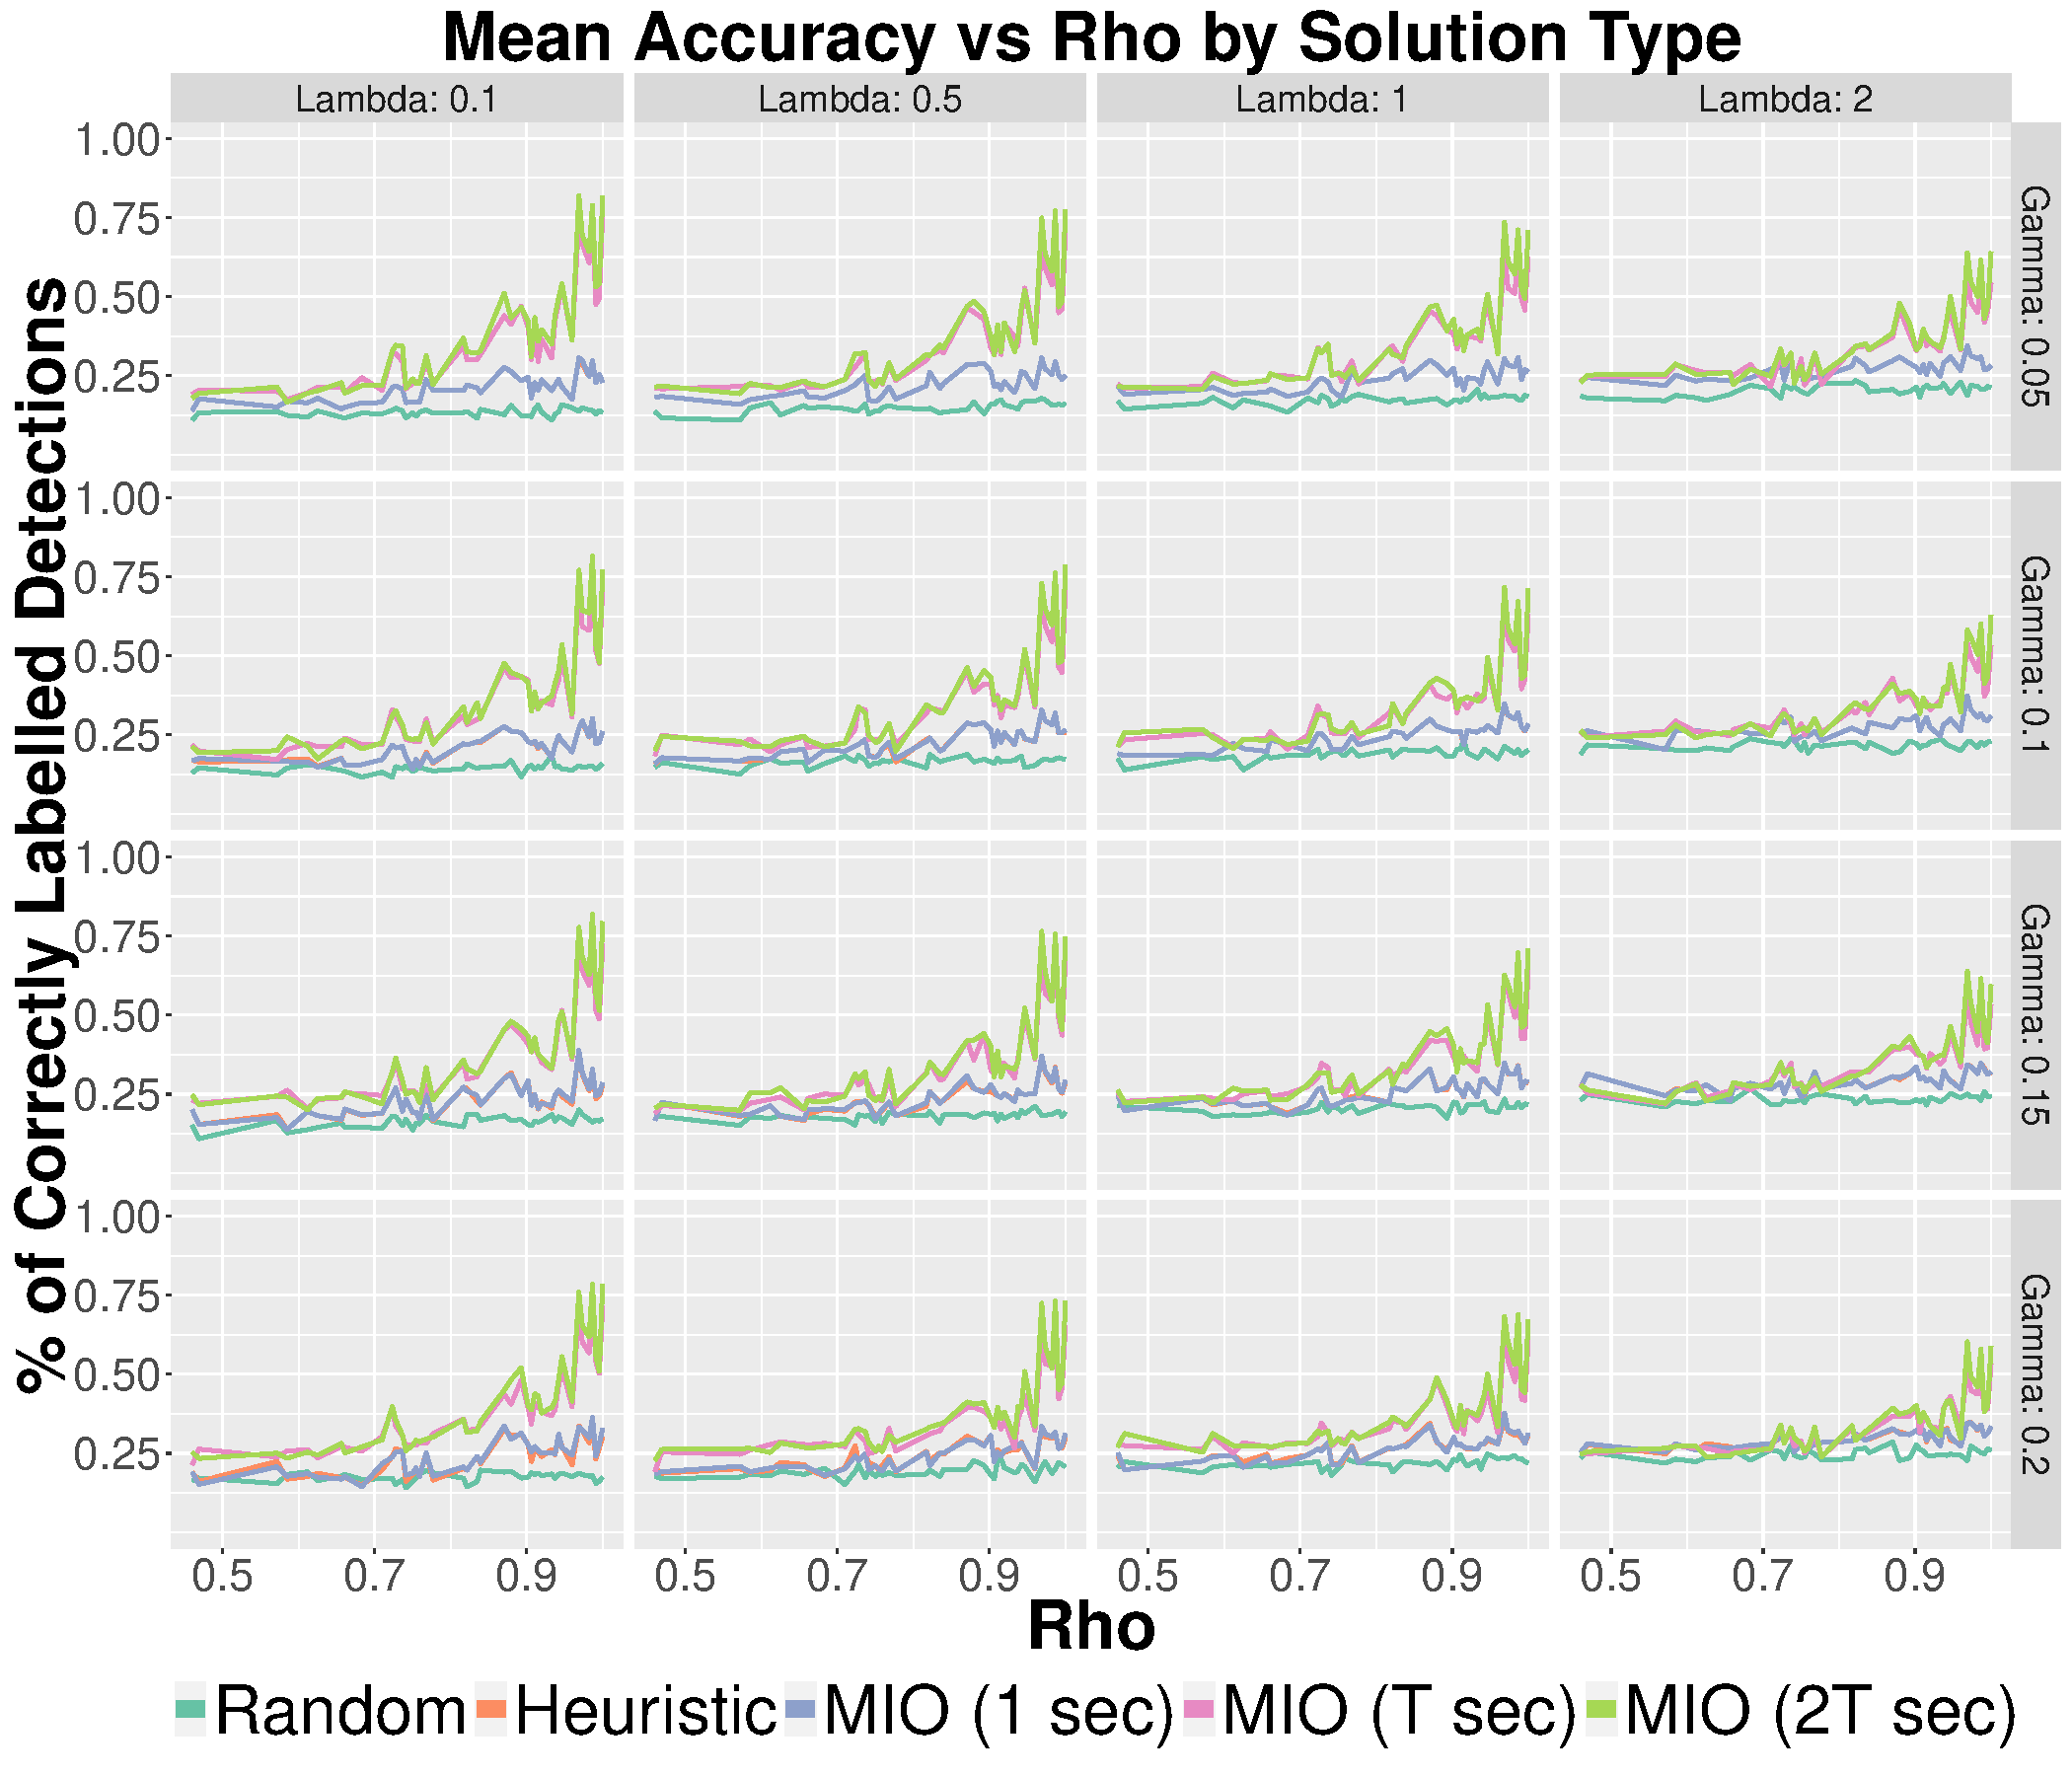
\includegraphics[width=9cm, height=7cm]{8_8_Accuracy}
  \caption{Accuracy of robust heuristic and MIO as compared to random solutions for scenarios of 8 targets and 8 scans, arranged by $\gamma$ and $\lambda$.}
  \label{fig:Robust_8_8_Accuracy}
\end{figure}

Similar to the performance of the basic heuristic, we again see that the robust heuristic improves greatly over that of a random solution, and the MIO offers even further improvement. Again, we seeing that running the MIO for 1 second offers significant improvements over the heuristic, and running the MIO for T seconds offers further improvement. However, running the MIO for 2T seconds offers little to no further improvement. Again, these results support the use of the MIO in an online algorithm with a sliding window as mentioned previously. 

Comparing Figure~\ref{fig:Robust_4_8_Accuracy} with the 4 target and 8 scan element of Figure~\ref{fig:Basic_Accuracy_Summary}, we see only a slight decrease in performance when $\gamma = 0.05$ and $\lambda=0.1$. This is an important result because we no longer know the number of targets in the robust case, yet we achieve almost the same levels of accuracy. Furthermore, both Figure~\ref{fig:Robust_4_8_Accuracy} and Figure~\ref{fig:Robust_8_8_Accuracy} show that the robust algorithms are more robust to decreases in the detection probability $\gamma$ than to increases in the false alarm rate $\lambda$. We conclude that the robust approaches are more sensitive to changes in the false alarm rate, in particular when it comes to making data associations. 

We have shown that both the heuristic and the MIO tend to underestimate the number of targets, due to the chosen penalties. We have also shown that accuracy degrades as the false alarm rate increases. This is likely not a coincidence. It is probable that as a result of underestimation, in which fewer trajectories are generated, there is a higher rate of misclassification of detections as false alarms, which in turn directly leads to a reduced accuracy. Therefore, it is a promising result to see accuracies above 75\% in Figure~\ref{fig:Robust_8_8_Accuracy}, even when Figure~\ref{fig:Robust_8_8_Histogram} suggests overestimation. It is entirely possible that further parameter tuning or introducing more complex penalties would lead to even great performance in the data association problem.

\subsubsection{Trajectory Estimation}
We conclude our analysis of the robust approaches with a discussion on their performance in the sphere of the trajectory estimation problem. Figures~\ref{fig:Robust_4_8_Delta} and~\ref{fig:Robust_8_8_Delta} plot the $\delta$ performance metric against the difficulty metric, $\sigma$, for scenarios of four and eight targets, respectively. Again, both scenarios have eight scans and both Figures have been arranged by $\gamma$ and $\lambda$. Note that the range on $\sigma$ has been reduced from $[0.1,5.0]$ to $[0.1, 2.0]$. 

\begin{figure}[h]
  \centering
  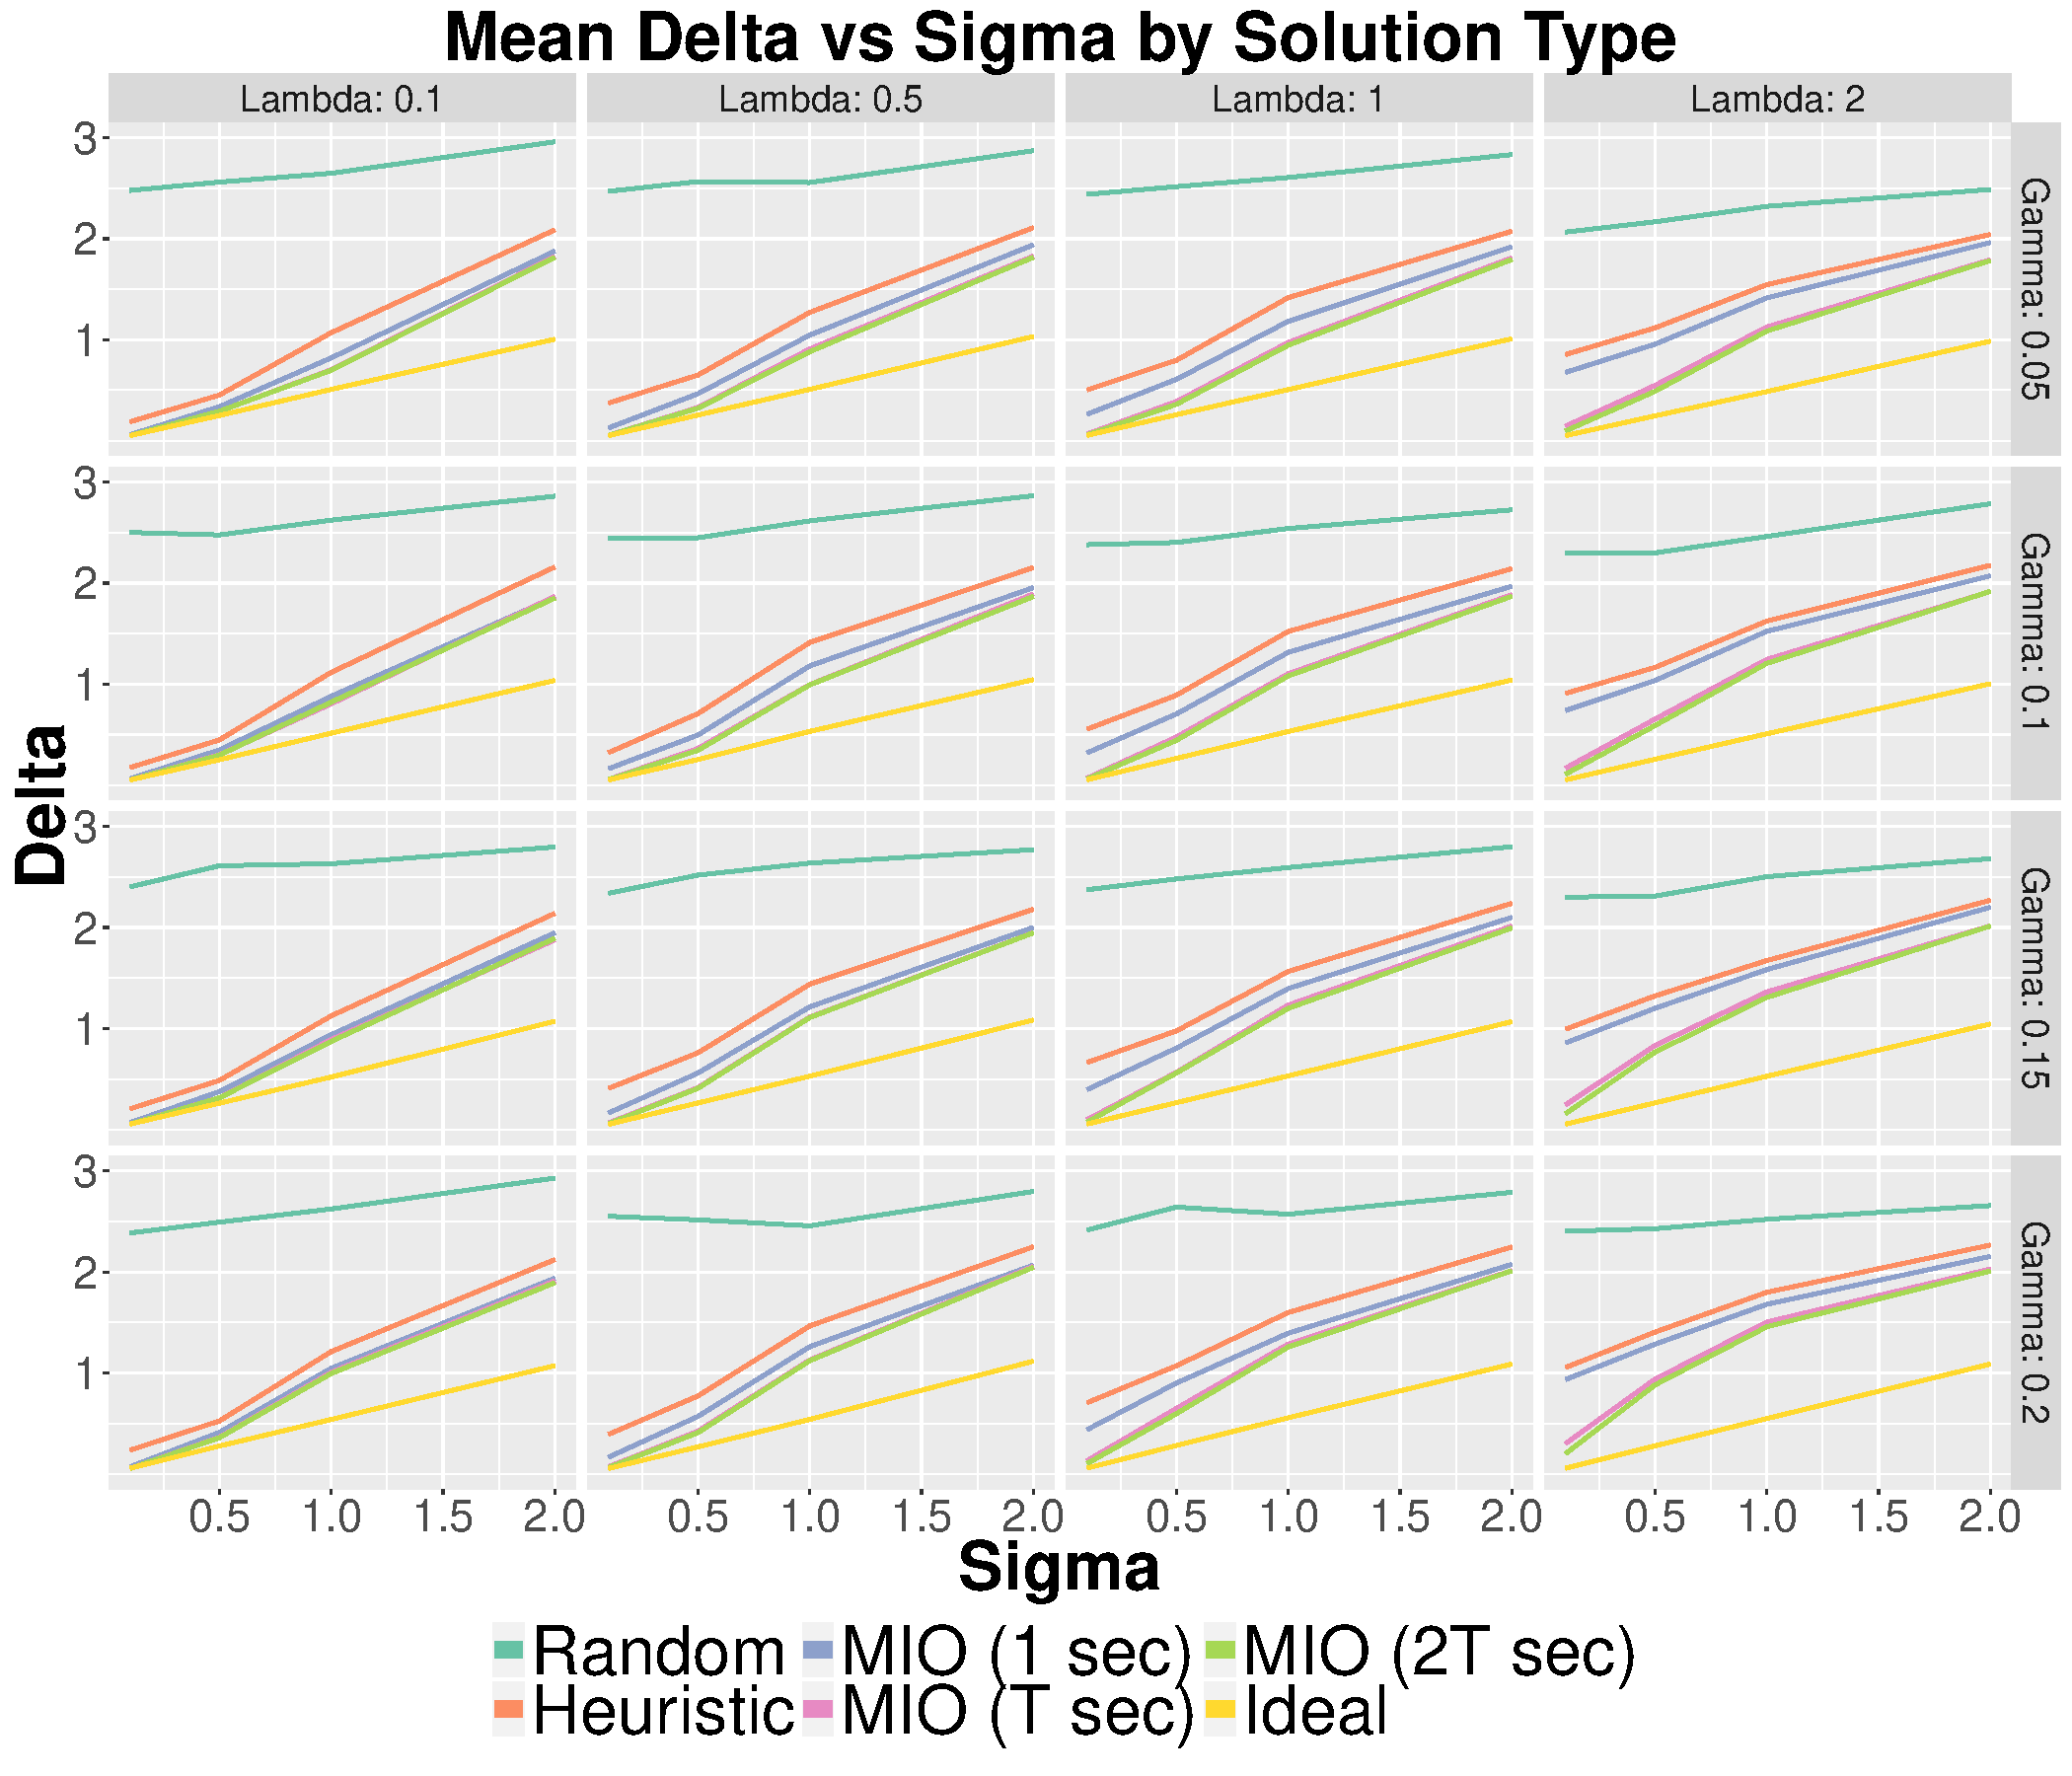
\includegraphics[width=9cm, height=7cm]{4_8_Delta}
  \caption{$\delta$ of robust heuristic and MIO as compared to random solutions for scenarios of 4 targets and 8 scans.}
  \label{fig:Robust_4_8_Delta}
\end{figure}

\begin{figure}[h]
  \centering
  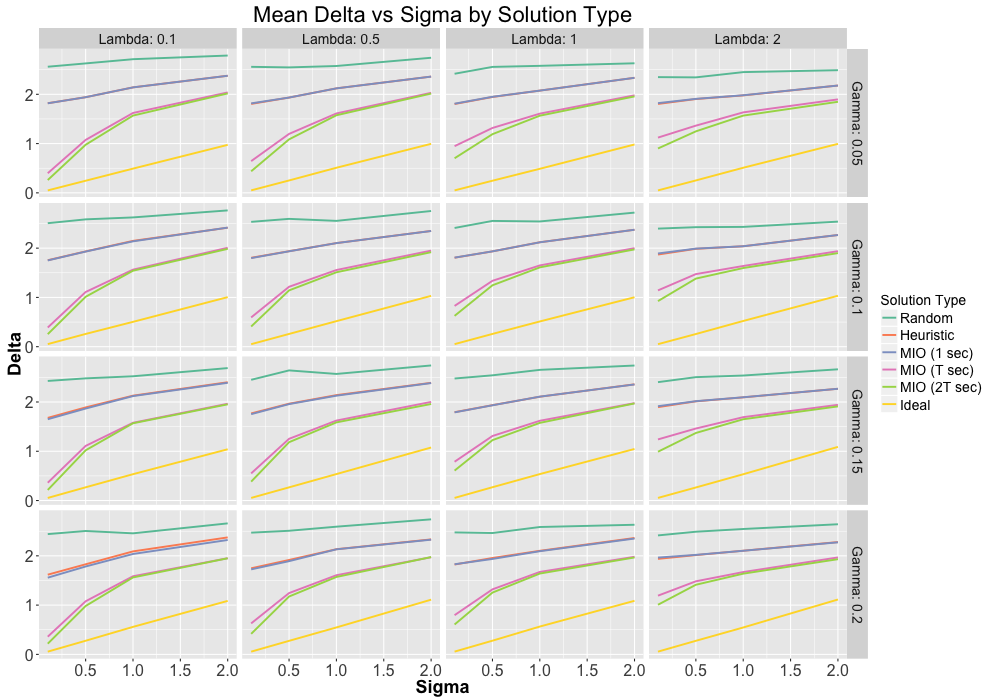
\includegraphics[width=9cm, height=7cm]{8_8_Delta}
  \caption{$\delta$ of robust heuristic and MIO as compared to random solutions for scenarios of 8 targets and 8 scans.}
  \label{fig:Robust_8_8_Delta}
\end{figure}

Again, we measure against the basic approaches by comparing Figure~\ref{fig:Robust_4_8_Delta} with the 4 target and 8 scan element of Figure~\ref{Fig:Basic_Delta_Summary}. We see that the robust approaches do not drastically reduce in performance for the easiest robust scenario of $\gamma = 0.05$ and $\lambda = 0.1$. However, the gap in performance between the ideal solution and the solutions of the robust algorithms grows wider with increases in $\sigma$, something that is expected but was not as sizable in the basic experiment. Therefore, the robust approaches may be less robust to increases in $\sigma$ in scenarios with detection ambiguity. However, it also appears that these methods are more robust to increases in the false alarm rate $\lambda$ when it comes to trajectory estimation than they were when it came to data association, especially in the larger scenario shown in Figure~\ref{fig:Robust_8_8_Delta}. We conclude that our robust methods are fairly robust to both increases in the false alarm rate and decreases in trajectory estimation under detection ambiguity, but increasing the signal noise degrades the performance of our methods more so in scenarios with detection ambiguity than in scenarios without detection ambiguity.

\section{Conclusion and Future Work}\label{sec:Conclusion}
We presented multi-target tracking approaches which jointly solve the problems of data association and trajectory estimation via global optimization methods using a single objective function. To this end, we proposed the use of a randomized local search heuristic as a warmstart for a mixed integer optimization model, and we did so for scenarios with and without detection ambiguity. We accomplish this without the need of a trajectory bank nor the a prior computation of trajectory hypotheses. We demonstrated that the proposed methods. Possible areas of future work could explore extensions to an online algorithm with a sliding window or extensions which account for the birth/death of targets. Additionally, future research could explore the use of more complex penalty functions through the addition of piecewise linear constraints. 

\appendices
\section{Estimated Trajectory Assignments}\label{sec:Assignment_Appendix}
In order to analyze the performance of a multi-target tracking algorithm, we must find the best matching of the true trajectories of the scenario and the estimated trajectories of the algorithm solution. Put differently, we wish to find a set of assignment pairings which match true and estimated trajectories. Here we present a linear optimization model which solves for the globally optimal assignment pairings of true and estimated trajectories. In addition, we discuss the required 

The goal of this assignment problem is to optimally assign pairs of true trajectories \textit{i} to estimated trajectories \textit{j} if there exists such a pairing to be made. Only a single set of decision variables are needed to determine if the true trajectory \textit{i} should be assigned to the estimated trajectory \textit{j} or not. 
\[y_{ij} = 
\begin{cases}
1, & \text{if true trajectory \textit{i} is assigned}\\
    & \text{ to estimated trajectory \textit{j},}\\
0, & \text{otherwise.}
\end{cases}\]

Remember that we denote the true position of trajectory \textit{i} at scan \textit{t} with $\bar{x}_{it}$ and the estimated position of trajectory \textit{j} at scan \textit{t} with $\hat{x}_{jt}$. Then the cost $c_{ij}$ of assigning true trajectory \textit{i} to estimated trajectory \textit{j} is the norm distance between these two trajectories as measured at each scan. 
\begin{align}
	c_{ij} = \sum_{t=1}^{T} \|\bar{x}_{it} - \hat{x}_{jt}\|
\end{align}

If we denote the true number of targets as $P_{\text{true}}$ and the estimated number of targets as $P_{\text{estimated}}$ then the objective of the integer optimization model would be:
\begin{align}
\underset{y_{ij}}{\text{minimize: }} & \sum_{i=1}^{P_{\text{true}}} \sum_{j=1}^{P_{\text{estimated}}} c_{ij}y_{ij}
\end{align}

When the number of true targets is equal to the number of estimated targets ($P_{\text{true}} = P_{\text{estimated}} = P$), we simply require two equality constraints to ensure that each true trajectory \textit{i} is assigned to exactly one estimated trajectory \textit{j} and vice versa. 
\begin{align}\label{eqn:assignment_1}
\sum_{i=1}^{P} y_{ij} = 1 \qquad \forall j = 1,...,P
\end{align}

\begin{align}\label{eqn:assignment_2}
\sum_{j=1}^{P} y_{ij} = 1 \qquad \forall i = 1,...,P
\end{align}

However, when the number of estimated trajectories differs from the number of true trajectories, these constraints must be modified slightly. In the case where the number of true targets exceeds the estimated number of targets ($P_{\text{true}}\geq P_{\text{estimated}}$), we restrict each true trajectory \textit{i} to the assignment of \textit{at most} one estimated trajectory \textit{j}, and Equation~\ref{eqn:assignment_1} is modified to
\begin{align}
\sum_{i=1}^{P_{\text{true}}} y_{ij} \leq 1 \qquad \forall  j = 1,...,P_{\text{estimated}}
\end{align}

On the contrary, when the number of estimated targets exceeds the true number of targets ($P_{\text{true}}\leq P_{\text{estimated}}$), then we restrict each estimated trajectory \textit{j} to the assignment of \textit{at most} one true trajectory \textit{i}, and Equation~\ref{eqn:assignment_2} is modified to
\begin{align}
\sum_{j=1}^{P_{\text{estimated}}} y_{ij} \leq 1 \qquad \forall i = 1,...,P_{\text{true}}
\end{align}

In summary, the generalized integer optimization assignment model is presented below.  
\begin{align*}
\underset{y_{ij}}{\text{minimize: }} & \sum_{i=1}^{P_{\text{true}}} \sum_{j=1}^{P_{\text{estimated}}} c_{ij}y_{ij}\\
\text{subject to: }	& \sum_{i=1}^{P_{\text{true}}} y_{ij} = 1 \qquad \forall j = 1,...,P_{\text{estimated}}\\
				& \sum_{j=1}^{P_{\text{estimated}}} y_{ij} = 1 \qquad \forall i = 1,...,P_{\text{true}}\\
				& y_{ij} \in \{0,1\} \quad \forall i = 1,...,P_{\text{true}},j = 1,...,P_{\text{estimated}}
\end{align*}

\section{Experiment 2 Penalty Values}\label{sec:Penalty_Appendix}
Here we provide recommendations for the tuning of penalty parameters $\theta$ and $\phi$. We begin with an explanation of grounded in logic. It can be shown that as the false alarm rate $\lambda$ increases, the number of expected false alarms also increases. Therefore, it stands to reason that as a general rule of thumb the false alarm penalty $\theta$ should decrease as $\lambda$ increases. Similarly, the number of expected missed detections increases as the missed detection probability $\gamma$ increases, and so too the missed detection penalty should decrease. Then it follows logically that the missed detection penalty $\phi$ should increase as $\gamma$ decreases. Furthermore, it is convenient to reason that the value of both of these penalties should somehow be tied to the value of $\sigma$, though this is a more difficult sequence of logic to justify. Through examination we found these logical concepts to hold true across a variety of scenario sizes and difficulties. Using this insight as well as the results of a mini experiment, we arrived at the penalty values summarized in Table~\ref{tab:Penalties} below. 

\begin{table}[ht]
\centering
\begin{tabular}{c|c|c|c|c}
\hline
$\sigma$ & $\gamma$ & $\lambda$ & $\theta$ & $\phi$\\
\hline
0.1 & 0.2 & 0.1 & 0.4 & 0.1 \\
0.1 & 0.2 & 0.5 & 0.2 & 0.1 \\
0.1 & 0.2 & 1.0 & 0.3 & 0.2 \\
0.1 & 0.2 & 2.0 & 0.1 & 0.2 \\
0.1 & 0.15 & 0.1 & 0.4 & 0.1 \\
0.1 & 0.15 & 0.5 & 0.4 & 0.1 \\
0.1 & 0.15 & 1.0 & 0.4 & 0.3 \\
0.1 & 0.15 & 2.0 & 0.1 & 0.3 \\
0.1 & 0.1 & 0.1 & 0.3 & 0.1 \\
0.1 & 0.1 & 0.5 & 0.3 & 0.2 \\
0.1 & 0.1 & 1.0 & 0.2 & 0.2 \\
0.1 & 0.1 & 2.0 & 0.1 & 0.3 \\
0.1 & 0.05 & 0.1 & 0.3 & 0.2 \\
0.1 & 0.05 & 0.5 & 0.2 & 0.2 \\
0.1 & 0.05 & 1.0 & 0.1 & 0.4 \\
0.1 & 0.05 & 2.0 & 0.1 & 0.4 \\
0.5 & 0.2 & 0.1 & 0.5 & 0.1 \\
0.5 & 0.2 & 0.5 & 0.4 & 0.2 \\
0.5 & 0.2 & 1.0 & 0.4 & 0.2 \\
0.5 & 0.2 & 2.0 & 0.3 & 0.3 \\
0.5 & 0.15 & 0.1 & 0.5 & 0.1 \\
0.5 & 0.15 & 0.5 & 0.4 & 0.2 \\
0.5 & 0.15 & 1.0 & 0.4 & 0.3 \\
0.5 & 0.15 & 2.0 & 0.3 & 0.4 \\
0.5 & 0.1 & 0.1 & 0.4 & 0.3 \\
0.5 & 0.1 & 0.5 & 0.4 & 0.3 \\
0.5 & 0.1 & 1.0 & 0.3 & 0.3 \\
0.5 & 0.1 & 2.0 & 0.2 & 0.4 \\
0.5 & 0.05 & 0.1 & 0.4 & 0.4 \\
0.5 & 0.05 & 0.5 & 0.4 & 0.4 \\
0.5 & 0.05 & 1.0 & 0.3 & 0.5 \\
0.5 & 0.05 & 2.0 & 0.3 & 0.5 \\
1.0 & 0.2 & 0.1 & 0.5 & 0.1 \\
1.0 & 0.2 & 0.5 & 0.5 & 0.2 \\
1.0 & 0.2 & 1.0 & 0.5 & 0.1 \\
1.0 & 0.2 & 2.0 & 0.5 & 0.4 \\
1.0 & 0.15 & 0.1 & 0.5 & 0.1 \\
1.0 & 0.15 & 0.5 & 0.5 & 0.3 \\
1.0 & 0.15 & 1.0 & 0.5 & 0.2 \\
1.0 & 0.15 & 2.0 & 0.5 & 0.4 \\
1.0 & 0.1 & 0.1 & 0.5 & 0.5 \\
1.0 & 0.1 & 0.5 & 0.5 & 0.4 \\
1.0 & 0.1 & 1.0 & 0.4 & 0.4 \\
1.0 & 0.1 & 2.0 & 0.4 & 0.5 \\
1.0 & 0.05 & 0.1 & 0.5 & 0.5 \\
1.0 & 0.05 & 0.5 & 0.5 & 0.5 \\
1.0 & 0.05 & 1.0 & 0.5 & 0.5 \\
1.0 & 0.05 & 2.0 & 0.5 & 0.5 \\
2.0 & 0.2 & 0.1 & 0.5 & 0.1 \\
2.0 & 0.2 & 0.5 & 0.5 & 0.2 \\
2.0 & 0.2 & 1.0 & 0.5 & 0.1 \\
2.0 & 0.2 & 2.0 & 0.5 & 0.5 \\
2.0 & 0.15 & 0.1 & 0.5 & 0.1 \\
2.0 & 0.15 & 0.5 & 0.5 & 0.3 \\
2.0 & 0.15 & 1.0 & 0.5 & 0.2 \\
2.0 & 0.15 & 2.0 & 0.5 & 0.5 \\
2.0 & 0.1 & 0.1 & 0.5 & 0.5 \\
2.0 & 0.1 & 0.5 & 0.5 & 0.5 \\
2.0 & 0.1 & 1.0 & 0.5 & 0.5 \\
2.0 & 0.1 & 2.0 & 0.5 & 0.5 \\
2.0 & 0.05 & 0.1 & 0.5 & 0.5 \\
2.0 & 0.05 & 0.5 & 0.5 & 0.5 \\
2.0 & 0.05 & 1.0 & 0.5 & 0.5 \\
2.0 & 0.05 & 2.0 & 0.5 & 0.5 \\
\hline
\end{tabular}
\caption{Experiment 2 penalty values.}
\label{tab:Penalties}
\end{table}

\section*{Acknowledgments}
The authors would like to thank Sung-Hyun Son, Ph.D. and Steven Relyea at Lincoln Laboratories for introducing us to the MTT problem and for their ongoing guidance throughout this work. Additionally, we would like to thank Lincoln Laboratories and the LLGrid team for their continual support in running our experiments. 

CONTRACT ACKNOWLEDGMENT: This material is based upon work supported by the Air Force under Air Force Contract No. FA8721-05-C-0002 and/or FA8702-15-D-0001. Any opinions, findings, conclusions or recommendations expressed in this material are those of the author(s) and do not necessarily reflect the views of the U.S. Air Force. 


% trigger a \newpage just before the given reference
% number - used to balance the columns on the last page
% adjust value as needed - may need to be readjusted if
% the document is modified later
%\IEEEtriggeratref{8}
% The "triggered" command can be changed if desired:
%\IEEEtriggercmd{\enlargethispage{-5in}}

% references section


% The IEEEtran BibTeX style support page is at:
% http://www.michaelshell.org/tex/ieeetran/bibtex/
%\nocite{*}
\bibliographystyle{IEEEtran}
% argument is your BibTeX string definitions and bibliography database(s)
\bibliography{Bibliography}
%

%\printbibliography

\end{document}